\documentclass[10pt, a4paper]{article}

% Packages
%======================================
% Page Geometry
\usepackage{geometry}
\geometry{a4paper, left=1in, right=1in, top=1in, bottom=1in, headheight=13.6pt}
%======================================
% Document spacing
% Line spacing
\usepackage{setspace}
\setstretch{1.2}
% Paragraph spacing
\usepackage[skip=2.5pt, indent=12pt]{parskip}
%======================================
% Headers and footnotes
\usepackage{fancyhdr}
%======================================
% Math packages
\usepackage{tikz}
% Norm command
\usepackage{physics}
\usepackage{tikz-cd}
\usepackage{mathtools}
\usepackage{amsmath,amssymb}
\newcommand\numberthis{\addtocounter{equation}{1}\tag{\theequation}}
% Inline fractions
\usepackage{nicefrac}
% Overbar that fits
\newcommand{\overbar}[1]{\mkern 1.5mu\overline{\mkern-1.5mu#1\mkern-1.5mu}\mkern 1.5mu}
% Quotient space
\newcommand{\bigslant}[2]{{\raisebox{.2em}{$#1$}\left/\raisebox{-.2em}{$#2$}\right.}}
% Array stretch for matrices
\makeatletter
\renewcommand*\env@matrix[1][\arraystretch]{%
  \edef\arraystretch{#1}%
  \hskip -\arraycolsep
  \let\@ifnextchar\new@ifnextchar
  \array{*\c@MaxMatrixCols c}}
\makeatother
%======================================
% Theorem environments
\usepackage{amsthm}
\newtheoremstyle{BoldTopBottomSpacing}
  {0.7em} % Space above
  {0.7em} % Space below
  {} % Body font
  {} % Indent amount
  {\bfseries} % Head font
  {.} % Punctuation after head
  {0.5em} % Space after head
  {} % Head spec
\newtheoremstyle{BoldTopSpacing}
  {0.7em}
  {\topsep}
  {\itshape}
  {}
  {\bfseries}
  {.}
  {0.5em}
  {}
% Theorem
\theoremstyle{BoldTopSpacing}
\newtheorem{theorem}{Theorem}[section]
% Lemma
\theoremstyle{BoldTopSpacing}
\newtheorem{lemma}[theorem]{Lemma}
% Corollary
\theoremstyle{BoldTopSpacing}
\newtheorem{corollary}{Corollary}[theorem]
% Definition
\theoremstyle{BoldTopBottomSpacing}
\newtheorem{definition}{Definition}[section]
% Proposition
\theoremstyle{BoldTopSpacing}
\newtheorem{proposition}{Proposition}[section]
% Example
\theoremstyle{BoldTopBottomSpacing}
\newtheorem{example}{Example}[section]
% Remark
\theoremstyle{remark}
\newtheorem{remark}{\textit{Remark}}[section]
% Sketch of proof
\newenvironment{proofsketch}{%
  \renewcommand{\proofname}{Proof sketch}\proof}{\endproof}
%======================================
% German ß ä ö ü
\usepackage{lmodern}
\usepackage[T1]{fontenc}
\usepackage[main=english,german]{babel}
%======================================
% Quotation marks
\usepackage{csquotes}
%======================================
% Lists
\usepackage{enumitem}
%======================================
% Color
\usepackage{xcolor}
\definecolor{TUColor}{cmyk}{0, 1.0, 0.99, 0.40} % TU Dark Red
\definecolor{CitationColor}{cmyk}{0.9, 0.6, 0.0, 0.6} % Dark Blue
\definecolor{RichBlack}{cmyk}{0.75, 0.68, 0.67, 0.9}
%======================================
% Hyper links and references
\usepackage{hyperref}
\hypersetup{
    colorlinks,
    urlcolor={CitationColor},
    citecolor={CitationColor},
    linkcolor={RichBlack}
}
%======================================
% Citations
\usepackage[nobreak]{cite}
% Define cites command for multiple citations
\makeatletter
\newcommand{\citecomment}[2][]{\citen{#2}#1\citevar}
\newcommand{\citeone}[1]{\citecomment{#1}}
\newcommand{\citetwo}[2][]{\citecomment[,~#1]{#2}}
\newcommand{\citevar}{\@ifnextchar\bgroup{;~\citeone}{\@ifnextchar[{;~\citetwo}{]}}}
\newcommand{\citefirst}{\@ifnextchar\bgroup{\citeone}{\@ifnextchar[{\citetwo}{]}}}
\newcommand{\cites}{[\citefirst}
\makeatother
%======================================
% Images
\usepackage{float}
\usepackage{graphicx}
\graphicspath{{./images/}}
% Captions
\usepackage{subcaption}
\renewcommand\thesubfigure{\roman{subfigure}}
%======================================
% For Title page
\usepackage{tabularx, booktabs}
%======================================
% Fancy boxes
\usepackage[most]{tcolorbox}
\tcbuselibrary{skins,breakable}
\newtcolorbox{mathbox}[2][]{breakable, sharp corners, boxrule=0mm, leftrule=2mm, boxsep=0mm, arc=0mm, outer arc=0mm, opacityframe=0}
%======================================


\begin{document}
%===========================================================
% General settings
% Font color
\color{RichBlack}
% Redefine header "fancy" style
\fancypagestyle{fancy}{
    \fancyhead{}
    \fancyfoot{}
    \fancyhead[LE,RO]{\footnotesize\itshape\nouppercase{\rightmark}}
    \fancyhead[LO,RE]{\footnotesize\itshape\nouppercase{\leftmark}}
    \fancyfoot[C]{\footnotesize\itshape\nouppercase\thepage}
    \renewcommand{\headrulewidth}{0.4pt}
    \renewcommand{\footrulewidth}{0.0pt}
}
\fancypagestyle{tocstyle}{
  \fancyhead{}
  \fancyfoot{}
  \renewcommand{\headrulewidth}{0.4pt}
  \renewcommand{\footrulewidth}{0.0pt}
}
%===========================================================


% Title page
%===========================================================
\begin{titlepage}
% Defines a new command for horizontal lines, change thickness here
\newcommand{\HRule}{\rule{\linewidth}{0.5mm}}
\begin{center}


\includegraphics[width=0.15\textwidth]{TU-Berlin-Logo.png}\\[1cm]
\begin{otherlanguage}{german}
\textsc{\LARGE Technische Universit"at Berlin}\\[1.5cm]
\textsc{\large Fakult\"at 2}\\[0.5cm]
\textsc{\large Institut f\"ur Mathematik}\\[0.5cm]
\end{otherlanguage}

% Title
\setlength{\aboverulesep}{10pt}
\setlength{\belowrulesep}{13pt}
\begin{tabularx}{\textwidth}{ >{\centering\arraybackslash}X}
\midrule[0.5mm]
\huge\bfseries Circular cross sections of quadrics\\
\midrule[0.5mm]
\end{tabularx}

\textsc{\large Bachelor Thesis}\\[1.5cm]

% Author and supervisor
\begin{minipage}{0.4\textwidth}
    \begin{flushleft}
        \large
        \textit{\textcolor{TUColor}{Author}}\\
        Sara \textsc{Samy}
    \end{flushleft}
\end{minipage}
~
\begin{minipage}{0.4\textwidth}
    \begin{flushright}
        \large
        \textit{\textcolor{TUColor}{Supervisor}}\\
        Dr. Jan \textsc{Techter}\\
        \large
        \textit{\textcolor{TUColor}{Second Supervisor}}\\
        Prof. Dr. Alexander \textsc{Bobenko}
    \end{flushright}
\end{minipage}

% Position the date 3/4 down the remaining page
\vspace{260 pt}
{\large\today}
\end{center}
\end{titlepage}
%===========================================================
% Set Abstract page style to "fancy"
\pagestyle{fancy}
\section*{Acknowledgement}
I would like to thank my supervisor Dr. Jan Techter for assigning me this topic, for his support and for many insightful discussions. I also would like to thank Prof. Dr. Alexander Bobenko for teaching me a lot about geometry and visualization. Overall, I am much indebted to the DDG working group at TU Berlin for their academic support, and for introducing me to many intriguing and beautiful topics in mathematics. \par
\pagebreak

\section*{}
\begin{otherlanguage}{german}
Hiermit erkl\"are ich, dass ich die vorliegende Arbeit selbstst\"andig und eigenh\"andig sowie ohne unerlaubte fremde Hilfe und ausschließlich unter Verwendung der aufgef\"uhrten Quellen und Hilfsmittel angefertigt habe. \par
Berlin, den \hrule
\end{otherlanguage}
\pagebreak
%===========================================================
% Set TOC page style to "tocstyle"
\pagestyle{tocstyle}
\renewcommand{\contentsname}{Contents}
\tableofcontents
\pagebreak
%===========================================================
\listoffigures
\pagebreak
%===========================================================
% Set all following pages style to "fancy"
\pagestyle{fancy}
\section{Introduction}
\label{sec:introduction}
Quadrics and their confocal families have played a prominent role in classical mathematics due to their elegant geometric properties and numerous applications across various domains, ranging from physics to art and architecture. \par
There are many ways to think about the geometry of quadrics. From the standpoint of differential geometry, quadrics \textemdash with the exception of quadratic cones, could be thought of as parameterized surfaces in $\mathbb{R}^3$, that is, maps $\varphi : \mathcal{U} \subseteq \mathbb{R}^2 \to \mathbb{R}^3$. Some assumptions of genericity are often made, such that the tangent vectors $\partial_{1} \varphi$ and $\partial_{2} \varphi$ are linearly independent in $\mathbb{R}^3$, or that all higher-order partial derivatives exist. The differential $\text{d}\varphi$ allows us to locally examine how a vector
\[
    x_{1} \frac{\partial}{\partial u} + x_{2} \frac{\partial}{\partial v}
\]
is pushed-forward to $\text{d}\varphi(x_{1}, x_{2})$. More concretely, the differential of $\varphi$ induces a metric
\[
    \boldsymbol{g}(x, y) := \langle \text{d}\varphi(x_{1}, x_{2}), \text{d}\varphi(y_{2}, y_{2}) \rangle
\]
which is a positive-definite inner product, and thus can be encoded by a symmetric matrix
\[
    (x, y) \mapsto x^\top \begin{pmatrix} E & F \\ F & G \end{pmatrix} y
\]
with $E = \left< \partial \varphi / \partial u, \partial \varphi / \partial u \right>$, $F = \left< \partial \varphi / \partial u, \partial \varphi / \partial v \right>$, and $G = \left< \partial \varphi / \partial v, \partial \varphi / \partial v \right>$. It's often useful \textemdash albeit not entirely correct, to think of $\boldsymbol{g}$ as a metric on the parameter domain $(u, v)$ itself. \par
An important invariant of a metric is its \textit{curvature}. One can study the curvature of a surface in terms of the normal curvatures $\kappa_{n}$ of the curves contained on it. The differential of the unit normal $\text{d}\boldsymbol{N}$ of the surface plays a key role here. The shape operator
\[
    S_{p} = - \text{d}\boldsymbol{N}_{p},
\]
which is a self-adjoint linear operator, encodes the maximum and minimum normal curvatures, denoted as $\kappa_{1}$ and $\kappa_{2}$, respectively, at a specific point on the surface. Additionally, its Eigenvectors are the tangential directions corresponding to these principal curvatures, known as the \textit{the principal directions}. A curve defined along principal directions of a surface is known as a \textit{curvature line}. In this setting, one can show that (non-singular, non-degenerate) quadrics are isothermal surfaces, that is, they admit an orthonormal parameterization along their curvature lines \cite{geometryIII}. \par
In other contexts, quadrics are usually defined as sets of points whose coordinates satisfy an equation of the second degree:
\[
    \sum_{i = 1}^3 a_i x_i^2 + \sum_{\substack{i, j = 1, i \neq j}}^3 a_{ij} x_i x_j + \underbrace{\sum_{i = 1}^3 b_i x_i}_{\text{linear terms}} + \underbrace{C}_{\text{constant term}}
\]
This can be an inconvenient definition, since a quadric and the set of points it defines are different objects. For instance, after such a definition all quadrics without points would be equal, and no distinction could be made between a hyperplane such $x = 0$, and a quadric $x^2 = 0$. It is therefore more convenient to define quadrics in a projective setting as a class $\{ \lambda b \}_{\lambda \in \mathbb{R} \setminus \{ 0 \}}$, where $b$ is a non-zero symmetric bilinear form. \par
Many properties of a given quadric can be defined in terms of its corresponding family of bilinear forms. For instance, associated with any bilinear form on a real $(n+1)$-dimensional vectorspace $V$ is a basis $\{e_1, \cdots, e_{n+1}\}$ such that $b(e_{i}, e_{j}) = 0$ for all $i \neq j$, and
\[
(e_i, e_j) = \begin{cases}
1 & 1 \leq i \leq p \\
-1 & p+1 \leq i \leq r \\
0 & r+1 \leq i \leq n+1.
\end{cases}
\]
If $\mathcal{Q}$ is a quadric represented by $b$, then the triple $(p, q := r-p, t := n+1-r)$ defines its \textit{signature}. This is crucial for the classification of quadrics. For instance, quadrics in complex projective space are projectively classifed by their ranks $r$, which may be understood to measure the degree of degeneration of the quadric. Checking the projective equivalence of two complex quadrics can thus be done just by comparing their ranks. Similarly, for the real case, two quadrics are projectively equivalent if they have the same rank $r$ and the same index $r - p$. \par

Both approaches to studying quadrics converge in the topic of confocal quadrics. Confocal quadrics are central to confocal coordinate systems, constituting a class of orthogonal coordinate systems, which is a classical theme in differential geometry. Recent work in \cite{DiscretizationConfocalQuadricsI} has introduced a novel characterization of confocal coordinate systems (See Theorem~\ref{thm:must-be-confocal}). Building on this work in \cites{MutuallyDiagonalNets2019}{geometryIII}, a parametrization for the lines of curvature on ellipsoids, where the diagonal coordinate lines form circles, was presented. It has been shown that any one-parameter family of confocal ellipsoids can be transformed to maintain congruent circular sections. \par
In this thesis, we extend these results of to one-sheeted and two-sheeted hyperboloids. The main claim is summarized as follows:
\begin{theorem}
\label{thm:main-result}
One- and two-sheeted hyperboloids exhibit the following properties.
\begin{itemize}
    \item Any hyperboloid can be sliced into two one-parameter families of circles.
    \item The net composed of the two families of circular cross sections of a hyperboloid and the net composed of its lines of curvature are mutually diagonal.
    \item There exists a deformation for hyperboloids, that is isometric along circular sections, preserving circles, curvature lines, and their diagonal relation.
\end{itemize}
\end{theorem}
\vspace{0.7em}
The proof of this claim is distributed throughout the thesis. In Section~(\ref{sec:circular-sections-of-quadrics}), we revisit the complex projective space and construct a model for Euclidean geometry using the notion of an absolute quadric. In \cite{bobenkoNonEuclideanLaguerreGeometry}, different geometries are presented as instances of the broader idea of a \textit{Cayley-Klein space}. This approach proves valuable in examining planar sections of quadrics, enabling the identification of circles on all non-singular and non-degenerate quadrics \textemdash excluding hyperbolic paraboloids. \par
Moving on to Section~(\ref{sec:confocal-quadrics}), we define confocal quadrics and discuss their geometric properties, which are essential for establishing confocal coordinate systems. \par
In Section~(\ref{sec:diagonally-related-nets}), we define the notion of diagonally-related nets on surfaces as introduced in \cite{MutuallyDiagonalNets2019}. Additionally, we present curvature line parameterizations for the one-sheeted and two-sheeted hyperboloids, demonstrating diagonal relation with their circular sections. \par
Section~(\ref{sec:isometric-deformation}) introduces a family of affine transformations that exhibit isometry along the circular sections of the one-sheeted and two-sheeted hyperboloids. As a result, we derive a one-parameter family of curvature line parametrizations for confocal hyperboloids, describing the isometric deformation of their circular cross sections. \par
The images in this thesis are created by me. Three-dimensional images are produced using \texttt{pyddg} library and rendered in Blender. Two dimensional illustrations are drawn using Inkscape. Some 2D illustrations are re-created from other sources referenced in the captions. The computer algebra system \texttt{SageMath} is used in proof of Proposition~\ref{prop:affine-transformation-two-hyperboloid}.
\pagebreak
%===========================================================
\section{Circular sections of quadrics}
\label{sec:circular-sections-of-quadrics}

Before we start investigating circles on quadrics, we recall a few facts about the $n$-dimensional complex projective space, and introduce Euclidean geometry as a subgeometry of projective geometry. \par

\subsection{The complex projective space $\mathbb{C}\mathbb{P}^n$}
\label{subsec:complex-projective-space}

A point in the complex projective space $\mathbb{C}\mathbb{P}^{n}$ is determined by $n + 1$ elements $(z_{0}, \dots, z_{n})$ of the field $\mathbb{C}$, not all simultaneously zero. Two $(n + 1)$-tuples $(z_{0}, \dots, z_{n})$ and $(z'_{0}, \dots, z'_{n})$ determine the same point if and only if there exists $\lambda \in \mathbb{C} \setminus \{ 0 \}$ such that $z_{i} = \lambda z_{i}'$ for $i = 0, \dots, n$. This defines an equivalence relation~$\sim$ on $\mathbb{C}^{n + 1} \setminus \{ 0 \}$, and we can identify the complex projective space $\mathbb{C}\mathbb{P}^n$ with the quotient space of $\mathbb{C}^{n + 1} \setminus \{ 0 \}$ under this equivalence relation:
\[
    \mathbb{C}\mathbb{P}^n \cong \bigslant{\left( \mathbb{C}^{n + 1} \setminus \{ 0 \} \right)}{\sim}.
\]
Any $(n+1)$-tuple defining a point $P$ is called a set of \textit{homogeneous coordinates} of $P$, and we write $P = [z_{0},\dots, z_{n}]$.\par

One way to express the equivalence relation on $\mathbb{C}^{n+1} \setminus \{ 0 \}$ is by stating that a linear subspace of dimension one in $\mathbb{C}^{n + 1}$ corresponds to a point in $\mathbb{C}\mathbb{P}^n$. Any $(k+1)$-dimensional linear subspace of $\mathbb{C}^{n + 1}$ can be similarly \enquote{projectivied} by associating to it a \textit{projective subspace} of $\mathbb{C}\mathbb{P}^n$ with projective dimension $k$.

\begin{definition}[]
\label{def:projective-subspace}
A $k$-dimensional projective subspace of $\mathbb{C}\mathbb{P}^n$ is a projective space $\mathbb{P}(U)$:
   \[
       \mathbb{P}(U) := \{ [z] \in \mathbb{C}\mathbb{P}^n : z \in U \}.
   \]
where $U$ is a $(k+1)$-dimensional linear subspace of $\mathbb{C}^{n+1}$.
\end{definition}

There are no arithmetic operations defined for points in a projective space, but we may use operations defined on linear subspaces to combine projective subspaces. \newline
If $\mathbb{P}(U_{1})$ and $\mathbb{P}(U_{2})$ are two projective subspaces, then their intersection or their \textit{meet }$ \mathbb{P}(U_{1}) \cap \mathbb{P}(U_{2})$ is the projective subspace $\mathbb{P}(U_{1} \cap U_{2})$, and we write
\[
\mathbb{P}(U_{1}) \wedge \mathbb{P}(U_{2}) := \mathbb{P}(U_{1} \cap U_{2}).
\]
Similarly, the projective span or the \textit{join} of $\mathbb{P}(U_{1})$ and $\mathbb{P}(U_{2})$ is the projective subspace $\mathbb{P}(U_{1} + U_{2})$, and we write
\[
\mathbb{P}(U_{1}) \vee \mathbb{P}(U_{2}) := \mathbb{P}(U_{1} + U_{2}).
\]

There is a natural embedding $\mathbb{C}^n \hookrightarrow \mathbb{C}\mathbb{P}^n$ which sends a point $(z_{0}, \dots, z_{n-1}) \in \mathbb{C}^n$ to its equivalent class $[z_{0},\dots, z_{n-1}, 1] \in \mathbb{C}\mathbb{P}^n$. This way we get all the \textit{affine points} of $\mathbb{C}\mathbb{P}^n$ with $z_{n} \neq 0$, since a point $[z_{0}, \dots, z_{n}]$ with $z_{n} \neq 0$ corresponds to the affine point $(z_{0}/z_{n}, \dots, z_{n-1}/z_{n}) \in \mathbb{C}^{n}$. The points of the complementary set with $z_{n} = 0$ are called \textit{points at infinity}. This notion depends on the choice of the coordinate $z_{n}$. In fact, $\mathbb{C}\mathbb{P}^n$ contains $n + 1$ isomorphic copies of the affine space $\mathbb{C}^n$:
\[
    U_{i} = \left\{ \left[ \frac{z_{0}}{z_{i}}, \dots, \frac{z_{n}}{z_{i}} \right] : z_{j} \in \mathbb{C} \ \text{for} \ j=0, \dots, n \ \text{and} \ z_{i} \neq 0 \right\} \cong \mathbb{C}^n, \quad \quad i=0, \dots, n.
\]
Every point in $\mathbb{C}\mathbb{P}^n$ is contained in at least one of these pieces, and can be written down in the affine coordinates of that piece [Figure~\ref{fig:affine-patches-diagram}].\par

\begin{figure}[H]
    \centering
    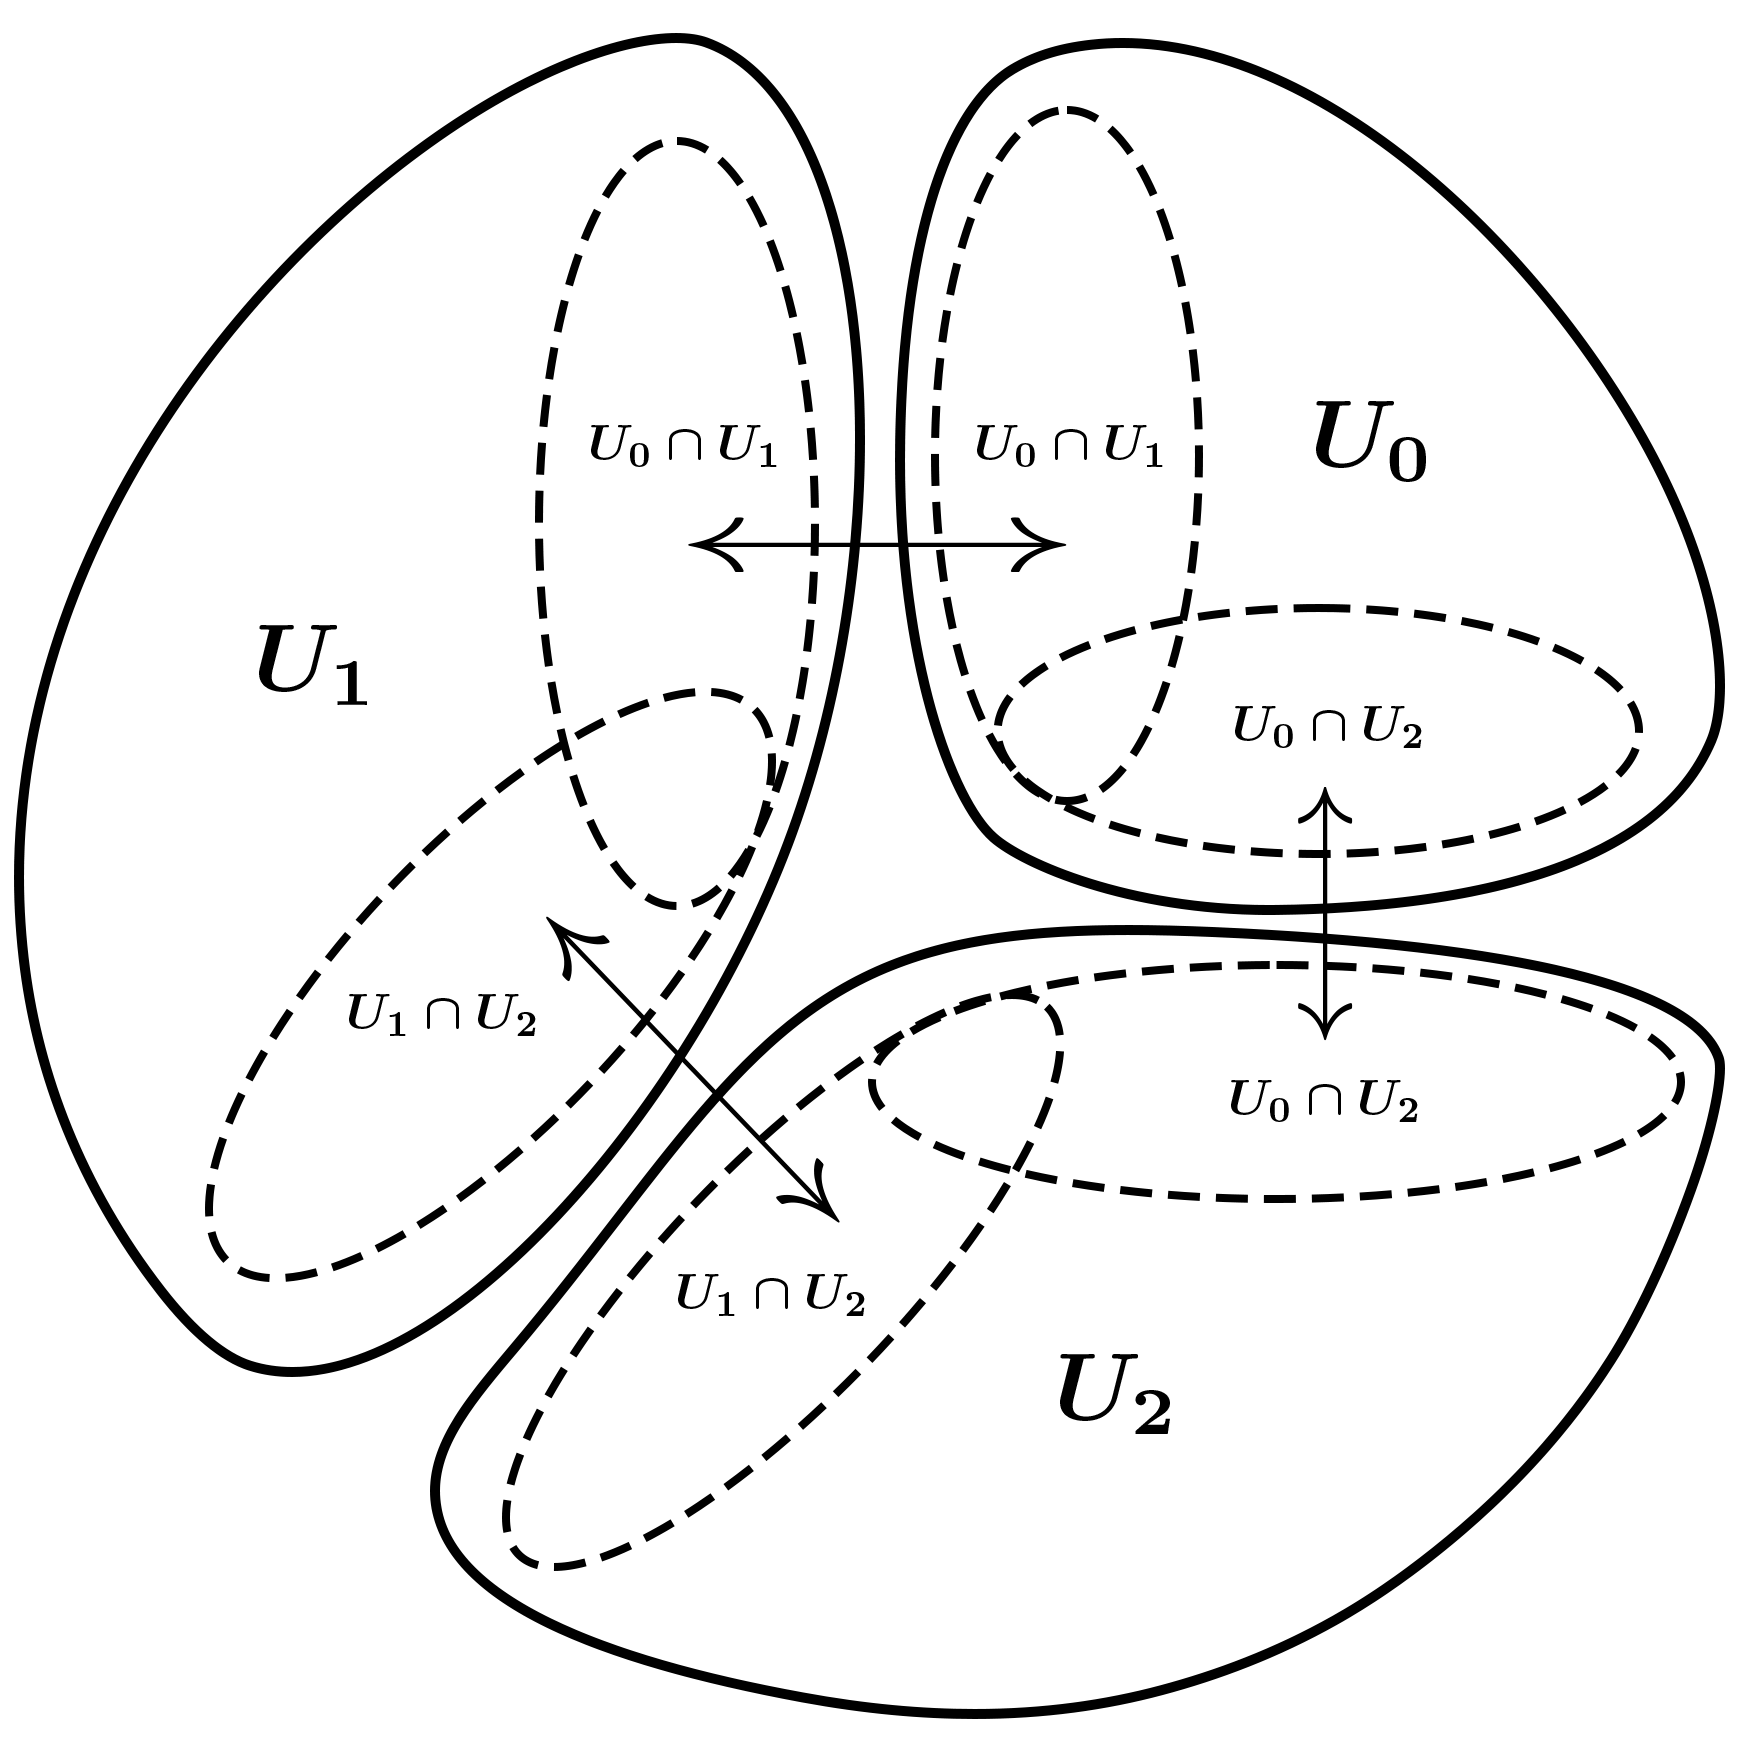
\includegraphics[width=0.5\textwidth]{affine-patches.png}
    \caption[$\mathbb{C}\mathbb{P}^2$ realised as the gluing of three affine patches $U_0, U_1$, and $U_2$.]{$\mathbb{C}\mathbb{P}^2$ realised as the gluing of three affine patches $U_0, U_1$, and $U_2$ \cite{toricfanovarieties2005}.}
    \label{fig:affine-patches-diagram}
\end{figure}

Once we have introduced homogeneous coordinates, we obtain another natural embedding of $\mathbb{R}\mathbb{P}^n$ into $\mathbb{C}\mathbb{P}^n$ by the map
\[
    \mathbb{R}\mathbb{P}^n \hookrightarrow \mathbb{C}\mathbb{P}^n, \quad \quad [x_{0}, \dots, x_{n}] \mapsto [x_{0}, \dots, x_{n}] \quad \text{for} \ x_{i} \in \mathbb{R}.
\]
A point $[z] \in \mathbb{C}\mathbb{P}^n$ is called \textit{real} if any of the following equivalent conditions are satisfed:
\begin{itemize}[label=$\blacktriangleright$]
    \item It lies in the image of the embedding map, i.e. $[z] \in \mathbb{R}\mathbb{P}^n$.
    \item It possesses a real representative in homogeneous coordinates, i.e. $[z] = [x_{0}, \dots, x_{n}]$ for $x_{i} \in \mathbb{R}$.
    \item It is equal to its complex conjugate point, i.e. $[z] = [\bar{z}]$.
\end{itemize}
Otherwise, it is called \textit{imaginary}. Note that a real point also has imaginary representatives: for instance, $[v] = [i v]$ for any non-zero $v \in \mathbb{R}^{n+1}$. Thus, the imaginary points are not simply those with an imaginary representative.

For a projective subspace $\mathbb{P}(U) \subset \mathbb{C}\mathbb{P}^n$, we define its \textit{real section} by
\[
    \mathbb{P}(U)_{\mathbb{R}} := \mathbb{P}(U \cap \mathbb{R}^{n+1}) = \mathbb{P}(U) \cap \mathbb{R}\mathbb{P}^n,
\]
which is the set of all the real points contained in $\mathbb{P}(U)$. The real section is necessarily a projective subspace, and its real dimension satisfes  $\text{dim}_{\mathbb{R}}\left(\mathbb{P}(U)_{\mathbb{R}}\right) \leq \text{dim}_{\mathbb{C}}\left(\mathbb{P}(U)\right)$ \cite{geometryII}.
Similarly, we define the \textit{complexification} of a projective subspace $\mathbb{P}(U) \subset \mathbb{R}\mathbb{P}^n$ as the complex span of its (real) points
\[
    \mathbb{P}(U)_{\mathbb{C}} := \mathbb{P}(\{ \lambda x + \gamma y \in \mathbb{C}^{n+1} : x, y \in U, \lambda, \gamma \in \mathbb{C} \}).
\]
The result of this complexification is also a projective subspace, whose complex dimension is equal to the real dimension of $\mathbb{P}(U)$ \cite{geometryII}. Thus, a projective subspace in $\mathbb{C}\mathbb{P}^n$ is \textit{real} if and only if $\mathbb{P}(U) = \mathbb{P}(U)_{\mathbb{R}}$. \par

\begin{proposition}[]
\label{thm:span-real-line}
An imaginary point $[z] \in \mathbb{C}\mathbb{P}^n$ is contained in exactly one real line, which is spanned by the points $[z]$ and $[\bar{z}]$.
\end{proposition}

\begin{proof}
The line $\ell = [z] \vee [\bar{z}]$ is a real line, since it's spanned by the two real points $[z + \bar{z}]$ and $[i(z - \bar{z})]$. If $[z]$ is contained in another real line $\tilde{\ell}$, then $z = \ell \wedge \tilde{\ell}$, which implies that it's a real point. Therefore, $[z]$ is contained in exactly one real line $\ell$.
\end{proof}

\subsection{The absolute quadric of Euclidean geometry}
\label{subsec:absolute-quadrics}

In the \textit{Klein Erlangen program}, Euclidean and non-Euclidean geometries are considered as subgeometries of projective geometry. Projective models for, e.g. hyperbolic, Euclidean, and spherical geometry are obtained by using a fundamental quadric to induce the corresponding metric. Every particular geometry deals with properties of figures in some space that remain invariant under some group of transformations of that space. These transformation groups can be regarded as subgroups of the projective linear group, that preserve the corresponding fundamental quadric. \par
In this section, we briefly introduce the notion of \textit{Cayley-Klein Distance} \cites[\textcolor{CitationColor}{Ch.~4}]{bobenkoNonEuclideanLaguerreGeometry}[\textcolor{CitationColor}{Ch.~9}]{geometryII}, \newline
which is used to derive an actual metric for a particular geometry. Then, we examine the construction of Euclidean geometry in that setting. \par

\begin{definition}
\label{def:cayley-klein-distance}
Let $\mathcal{Q}$ be a quadric in $\mathbb{R}\mathbb{P}^n$ with the corresponding bilinear form $b$. Then we denote by
\[
    K_{\mathcal{Q}}(x, y) := \frac{b(x, y)^2}{b(x, x) b(y, y)}
\]
the \textit{Cayley-Klein distance} of any two points $x, y \in \mathbb{R}\mathbb{P}^n \setminus \mathcal{Q}$ that are not on the quadric. Furthermore, we set $K_{\mathcal{Q}}(x, y) = \infty$ if $b(x, x) b(y, y) = 0$, and $b(x, y) \neq 0$. In the presence of a Cayley-Klein distance, the quadric $\mathcal{Q}$ is called the \textit{absolute quadric}.
\end{definition}

Note that the Cayley-Klein distance is projectively well-defined, in the sense that it depends neither on the choice of bilinear form corresponding to $\mathcal{Q}$ nor on the choice of homogeneous coordinates of $\mathbb{R}\mathbb{P}^n$. \par

\begin{remark}
\label{rm:isometries-cayley-klein}
\sloppy Let $f : \mathbb{R}\mathbb{P}^n \to \mathbb{R}\mathbb{P}^n$ denote a projective transformation, represented by a linear isomorphism ${ F : \mathbb{R}^{n+1} \to \mathbb{R}^{n+1} }$ that is orthogonal with respect to $\mathcal{Q}$, i.e.
\[
    b(F(X), F(Y)) = b(X, Y)
\]
for all $X, Y \in \mathbb{R}^{n + 1}$, and $f = [F]$. Then
\[
    K_{\mathcal{Q}}(f(x), f(y)) = K_{\mathcal{Q}}(x, y)
\]
for $x = [X], y = [Y] \in \mathbb{R}\mathbb{P}^n \setminus \{ Q \}$. The Cayley-Klein distance is invariant under the group of projective transformations that preserve the quadric $\mathcal{Q}$, which we call its corresponding group of \textit{isometries}. \par
\end{remark}

\subsubsection{The circular points of the Euclidean plane}
\label{subsubsec:circular-points-two-dimensional}

Let $\mathcal{Q}$ be a degenerate quadric with signature $(+ + 0)$ in the dual projective space $(\mathbb{R}\mathbb{P}^{2})^{*} \subset (\mathbb{C}\mathbb{P}^{2})^{*}$, and let $b$ denote its associated bilinear form
\[
    b(x, y) = x_{0}y_{0} + x_{1}y_{1}
\]
The equation of the quadric
\begin{equation*}
    \mathcal{Q} \; : \; x_{0}^2 + x_{1}^2 = 0
\end{equation*}
defines (upon complexification) two imaginary lines
\[
    \ell \; : \; x_{0} + i x_{1}, \quad \text{and} \quad \bar{\ell} \; : \; x_{0} - i x_{1}
\]
that intersect in a real point $\ell \wedge \bar{\ell} = [0, 0, 1]$. By duality, this real point corresponds to the line at infinity
\[
    \ell_{\infty} \; : \; x_{2} = 0
\]
in the primal space $\mathbb{R}\mathbb{P}^2$, whereas the two imaginary lines correspond to two complex conjugate points
\[
    \ell^{*} = [1, i, 0] \quad \text{and} \quad \bar{\ell}^{*} = [1, -i, 0]
\]
that lie on $\ell_{\infty}$. Thus, the dual quadric of $\mathcal{Q}$ is a non-degenerate imaginary quadric with signature $(+ +)$ contained entirely in $\ell_{\infty}$ \textemdash in other words, it consists only of two points
\begin{equation*}
    \mathcal{Z} = \left\{ [1, i, 0], [1, -i, 0] \right\}.
\end{equation*}

The two points $\ell^{*}$ and $\bar{\ell}^{*}$ of $\mathcal{Z}$ are known as the \textit{circular points at infinity}. The reason behind the naming is that, from a projective standpoint, these two imaginary points at infinity are contained in the complexification of every real circle. Indeed, circles are precisely conics through $\ell^{*}$ and $\bar{\ell}^{*}$ [Figure~\ref{fig:three-points-determine-a-circle}]. This gives some intuition to the fact that, e.g. only three non-collinear points uniquely determine a circle, whereas generically, five points are needed to determine a conic, or that the cocircularity of four points is (projectively) the coconicality of these four points with $\ell^{*}$ and $\bar{\ell}^{*}$. The next Theorem reformulates this idea. For a short proof, see \cite[\textcolor{CitationColor}{Proposition~9.9.}]{geometryII}. \par

\begin{theorem}
\label{thm:conic-through-circular-points}
A non-degenerate conic is a circle if and only if it contains the two circular points of $\mathcal{Z}$. Furthermore, the two imaginary tangent lines of a circle at the two circular points intersect in its center.
\end{theorem}

\begin{figure}[H]
    \centering
    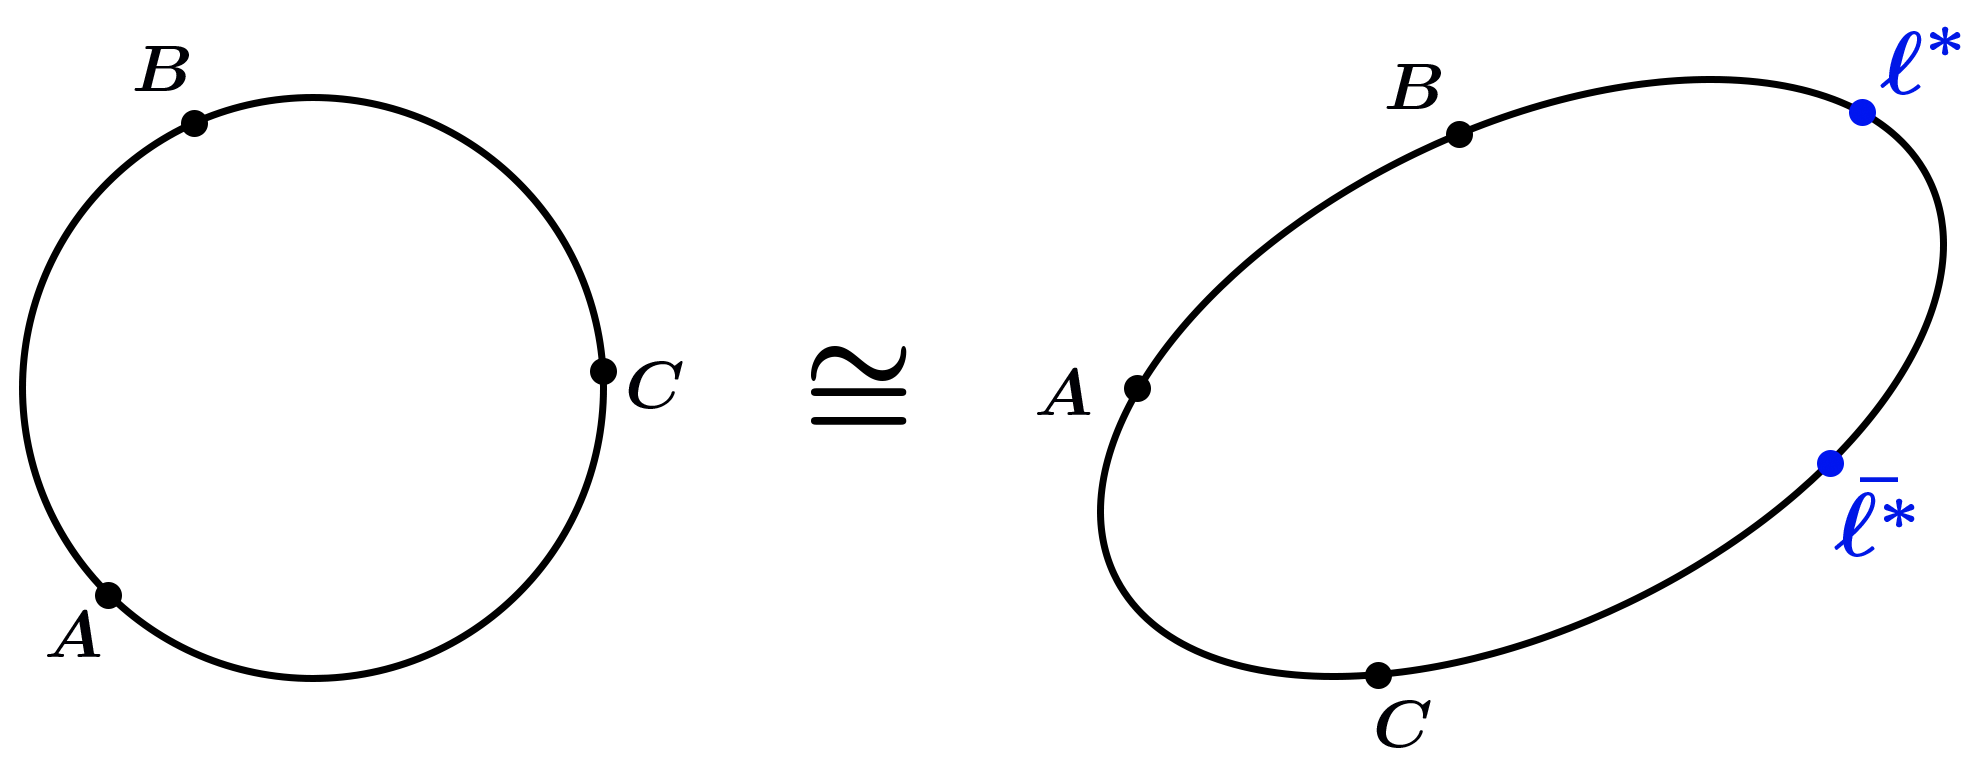
\includegraphics[width=0.6\textwidth]{three-points-determine-a-circle.png}
\caption[Circles are conics through the circular points at infinity.]{A real circle through the points $A, B$, and $C$ is (upon complexification) a conic through $A, B, C, \ell^{*}$, and $\bar{\ell}^{*}$ in $\mathbb{C}\mathbb{P}^2$.}
    \label{fig:three-points-determine-a-circle}
\end{figure}

\subsubsection{The absolute conic of Euclidean space}
\label{subsubsec:absolute-conic-three-dimensional}

Let $\mathcal{Q}$ be a degenerate quadric with signature $(+ + + 0)$ in the dual projective space $(\mathbb{R}\mathbb{P}^{3})^{*} \subset (\mathbb{C}\mathbb{P}^{3})^{*}$, and let $b$ denote its associated bilinear form
\[
    b(x, y) = x_{0} y_{0} + x_{1} y_{1} + x_{2} y_{2}.
\]
The equation of the quadric
\begin{equation}
\label{eq:degenerate-quadric-dual-space-three-dimensional}
    \mathcal{Q} \; : \; x_{0}^2 + x_{1}^2 + x_{2}^2 = 0
\end{equation}
defines (upon complexification) an imaginary cone, whose real part consists only of one point, namely its vertex $v := [0, 0, 0, 1]$ in homogeneous coordinates. Since $b(q, v) = 0$ for all points $q \in (\mathbb{R}\mathbb{P}^{3})^{*}$, the vertex is the only singular point of $Q$, and thus it has an \textit{undetermined} polar hyperplane, i.e. $H_{v} =  (\mathbb{R}\mathbb{P}^{3})^{*}$. \par
Let $p$ denote an arbitrary point on $\mathcal{Q} \setminus \{v\}$. Then, its polar hyperplane $H_{p}$ with respect to $\mathcal{Q}$ coincides with its tangent plane, since for any point $q \in H_{p}$ conjugate to $p$, the line $[p] \vee [q]$ is a tangent line to $Q$ at $p$. Moreover, this tangent plane necessarily passes through the vertex point. \par
If we dualize this construction, we find that the singular vertex point corresponds to the plane at infinity
\[
    H_{\infty} \; : \; x_{3} = 0
\]
in the primal space $\mathbb{R}\mathbb{P}^3$, whereas the tangent planes $H_{p}$ of $\mathcal{Q} \setminus \{v\}$ correspond to points that lie on $H_{\infty}$ and satisfy (\ref{eq:degenerate-quadric-dual-space-three-dimensional}) in homogeneous coordinates. Thus, the dual quadric of $Q$ is a non-degenerate imaginary conic with signature $(+ + +)$, that is entirely contained in the plane at infinity
\begin{equation}
\label{eq:absolute-conic}
\mathcal{Z} \; : \; x_{0}^2 + x_{1}^2 + x_{2}^2 = 0, \quad x_{3} = 0.
\end{equation}

This next Theorem is adapted from \cite[\textcolor{CitationColor}{Ch.~10}]{alveroAnalyticProjectiveGeometry}. Its statement is true for any $n$-dimensional projective space $\mathbb{R}\mathbb{P}^n \subset \mathbb{C}\mathbb{P}^n$, considered with its respective Euclidean absolute quadric. In fact, it implies Theorem~\ref{thm:conic-through-circular-points} in the two-dimensional case, where the absolute quadric is given by the circular points at infinity. We restrict ourselves to stating only the three-dimensional case here. \par

\begin{theorem}
\label{thm:quadrics-contain-absolute}
The quadrics in $\mathbb{R}\mathbb{P}^3 \subset \mathbb{C}\mathbb{P}^3$ that contain the absolute conic $\mathcal{Z}$ of Euclidean geometry \textemdash as constructed above, are:
\begin{itemize}[label=$\blacktriangleright$]
    \item spheres,
    \item imaginary spheres,
    \item cones with a real, affine vertex, and
    \item pairs of hyperplanes $H$ and $H_{\infty}$, where $H$ is an arbitrary hyperplane of $\mathbb{R}\mathbb{P}^3$.
\end{itemize}
\end{theorem}

\begin{proof}
Let $\mathcal{Q}$ denote a quadric in $\mathbb{R}\mathbb{P}^3 \subset \mathbb{C}\mathbb{P}^3$ with the homogeneous equation
\begin{equation}
    \mathcal{Q} \; : \; a_{0}x_{0}^2 + a_{1}x_{1}^2 + a_{2}x_{2}^2 + a_{3}x_{3}^2 + 2 \sum_{\substack{i = 1 \\ j < i}}^{3} a_{i, j} x_{i} x_{j} = 0,
\end{equation}
and $a_{i}, a_{i, j} \in \mathbb{R}$, not all zero. Then $\mathcal{Q}$ contains the absolute conic $\mathcal{Z}$ (\ref{eq:absolute-conic}) if and only if
\begin{equation*}
    a_{0}x_{0}^2 + a_{1}x_{1}^2 + a_{2}x_{2}^2 + 2 \sum_{\substack{i = 1 \\ j < i}}^{2} a_{i, j} x_{i} x_{j} = \lambda \left( x_{0}^2 + x_{1}^2 + x_{2}^2 \right)
\end{equation*}
for some $\lambda \in \mathbb{R}$ \cite[\textcolor{CitationColor}{Lemma~6.1.10.}]{alveroAnalyticProjectiveGeometry}. Thus, if $\mathcal{Q}$ contains the absolute conic, it must have equation of the form
\begin{equation}
\label{eq:quadrics-contain-absolute}
   \lambda \left( x_{0}^2 + x_{1}^2 + x_{2}^2 \right) + 2 \sum_{\substack{i = 0}}^{2} a_{i, 3} x_{i} x_{3} + a_{3} x_{3}^2 = 0.
\end{equation}
\par
If $\lambda = 0$, then equation (\ref{eq:quadrics-contain-absolute}) defines a pair of hyperplanes $H$ and $H_{\infty}$, where $H$ is an arbitrary hyperplane of $\mathbb{R}\mathbb{P}^3$ with affine equation
\[
    H \; : \; 2 \left( a_{0, 3} x_{0} + a_{1, 3} x_{1} + a_{2, 3} x_{2} \right) + a_{3} = 0.
\]
In particular, if $a_{i, 3} = 0$ for $i=0,1,2$, and $a_{3} \neq 0$, we get double copies of the plane at infinity
\[
    2 \; H_{\infty} \; : \; x_{3}^2 = 0.
\]
\par
If $\lambda \neq 0$, then $\mathcal{Q}$ does not contain $H_{\infty}$, but contains only the absolute conic as its section at infinity. We can rewrite the equation (\ref{eq:quadrics-contain-absolute}) as
\[
    x_{0}^2 + x_{1}^2 + x_{2}^2 + 2 \sum_{\substack{i = 0}}^{2} a'_{i} x_{i} x_{3} + a' x_{3}^2 = 0
\]
with $a'_{i} := a_{i, 3} / \lambda$, and $a' = a_{3} / \lambda$. Switching to affine coordinates and completing the squares, we get an equation of the form
\begin{equation}
\label{eq:real-or-imaginary-sphere}
(x_{0} - a'_{0})^2 + (x_{1} - a'_{1})^2  + (x_{2} - a'_{2})^2 = D,
\end{equation}
with $D := \sum_{i = 0}^{2} a'_{i} - a'$. The quadric $\mathcal{Q}$ it defines is degenerate if and only if $D = 0$, and in that case, $\mathcal{Q}$ is an imaginary cone over the absolute with real vertex given in affine coordinates by $(a'_{0}, a'_{1}, a'_{2})$. \par
If $D \neq 0$, then the quadric is non-degenerate, and we consider the two cases: If $D > 0$, then the equation (\ref{eq:real-or-imaginary-sphere}) is just the condition for an affine point $(x_{0}, x_{1}, x_{2})$ to be at distance $\sqrt{D}$ from the point $(a'_{0}, a'_{1}, a'_{2})$. Thus, the quadric $\mathcal{Q}$ is a sphere with center $(a'_{0}, a'_{1}, a'_{2})$ and radius $\sqrt{D}$. \par
If $D < 0$, then $\mathcal{Q}$ is a non-degenerate quadric with no real points, that intersects $H_{\infty}$ in the absolute conic $\mathcal{Z}$. Thus, we can call it an imaginary sphere with center $(a'_{0}, a'_{1}, a'_{2})$ and radius $\sqrt{D} = i \sqrt{-D}$.
\end{proof}

\begin{corollary}
\label{col:spheres-contain-absolute}
A non-degenerate quadric in $\mathbb{R}\mathbb{P}^3 \subset \mathbb{C}\mathbb{P}^3$ is a sphere if and only if it has real points and contains the absolute quadric $\mathcal{Z}$.
\end{corollary}

\subsection{Circles on quadrics}
\label{subsec:circles-on-quadrics}

Now we are ready to find circles on quadrics in $\mathbb{R}\mathbb{P}^3$. First, we note that circles are planar sections of spheres, and since any sphere contains the absolute conic $\mathcal{Z}$, it follows that a conic contained in a plane in $\mathbb{R}\mathbb{P}^3$ is a circle if and only if it intersects $\mathcal{Z}$ in two points. \par
Let $\mathcal{Q}$ be a non-degenerate, non-parabolic quadric in $\mathbb{R}\mathbb{P}^3$, and consider its restriction to the plane at infinity
\[
    H_{\infty} \; : \; x_{3} = 0.
\]
Let $\mathcal{C}$ denote this conic section at infinity. Then $\mathcal{C}$ intersects $\mathcal{Z}$ in four points, which are complex conjugate pairs $[z_{+}], [\bar{z}_{+}]$, and $[z_{-}], [\bar{z}_{-}]$. Together, they determine a complete quadrangle with three pairs of opposite lines:
\begin{align*}
    \ell_{1} &:= [z_{+}] \vee [\bar{z}_{+}] \quad \text{and} \quad \ell_{2} := [z_{-}] \vee [\bar{z}_{-}], \\
    \ell_{3} &:= [z_{+}] \vee [z_{-}] \quad \text{and} \quad \ell_{4} := [\bar{z}_{+}] \vee [\bar{z}_{-}], \; \text{and finally} \\
    \ell_{5} &:= [z_{+}] \vee [\bar{z}_{-}] \quad \text{and} \quad \ell_{6} :=  [z_{-}] \vee [\bar{z}_{+}]
\end{align*}
[Figure~\ref{fig:conics-through-four-points}]. However, only the first pair constitutes two real lines: $\ell_{1}$, and $\ell_{2}$, while the other two are pairs of imaginary lines \hyperref[thm:span-real-line]{(Proposition 2.1)}. Any plane through one of these lines, say $\ell_{1}$ intersects $\mathcal{Z}$ only at the corresponding complex conjugate points $[z_{+}]$ and $[\bar{z}_{+}]$, and thus, its intersection with $\mathcal{Q}$ (if non-empty) is necessarily a circle. By considering each pencil of planes determined by one of these lines (as its axis), we get all the circular sections of $\mathcal{Q}$. Note that the any such pencil is a pencil of parallel planes, since its planes intersect in a line at infinity. Therefore, there are three pairs of two pencils of parallel circular sections of $\mathcal{Q}$; one pair is real, and the others are imaginary. \par
If $\mathcal{Q}$ is a paraboloid with homogeneous equation $x_{0}^2 / a + x_{1}^2 / b - 2x_{2}x_{3} = 0$, then it intersects the plane at infinity $x_{3} = 0$ in two lines. In the case of an elliptical paraboloid, with $a, b > 0$, both of these lines are imaginary $x_{0}^2 / a + x_{1}^2 / b = 0$. However, their pencil of planes define real circular sections on the elliptical paraboloid. On the other hand, hyperbolic paraboloids intersect the plane at infinity in two real lines but they defines planes which cut the paraboloid in a line at infinity and another line. This pair form a degenerate case of a circle with centre at infinity. Thus, hyperbolic paraboloids possess no proper circular sections \cite[\textcolor{CitationColor}{p.~204}]{sommervilleAnalyticalGeometry}. \par

In the following Theorem, we compute the equations of the real pair of parallel circular sections in the case of two-sheeted hyperboloids.

\begin{figure}[H]
    \centering
    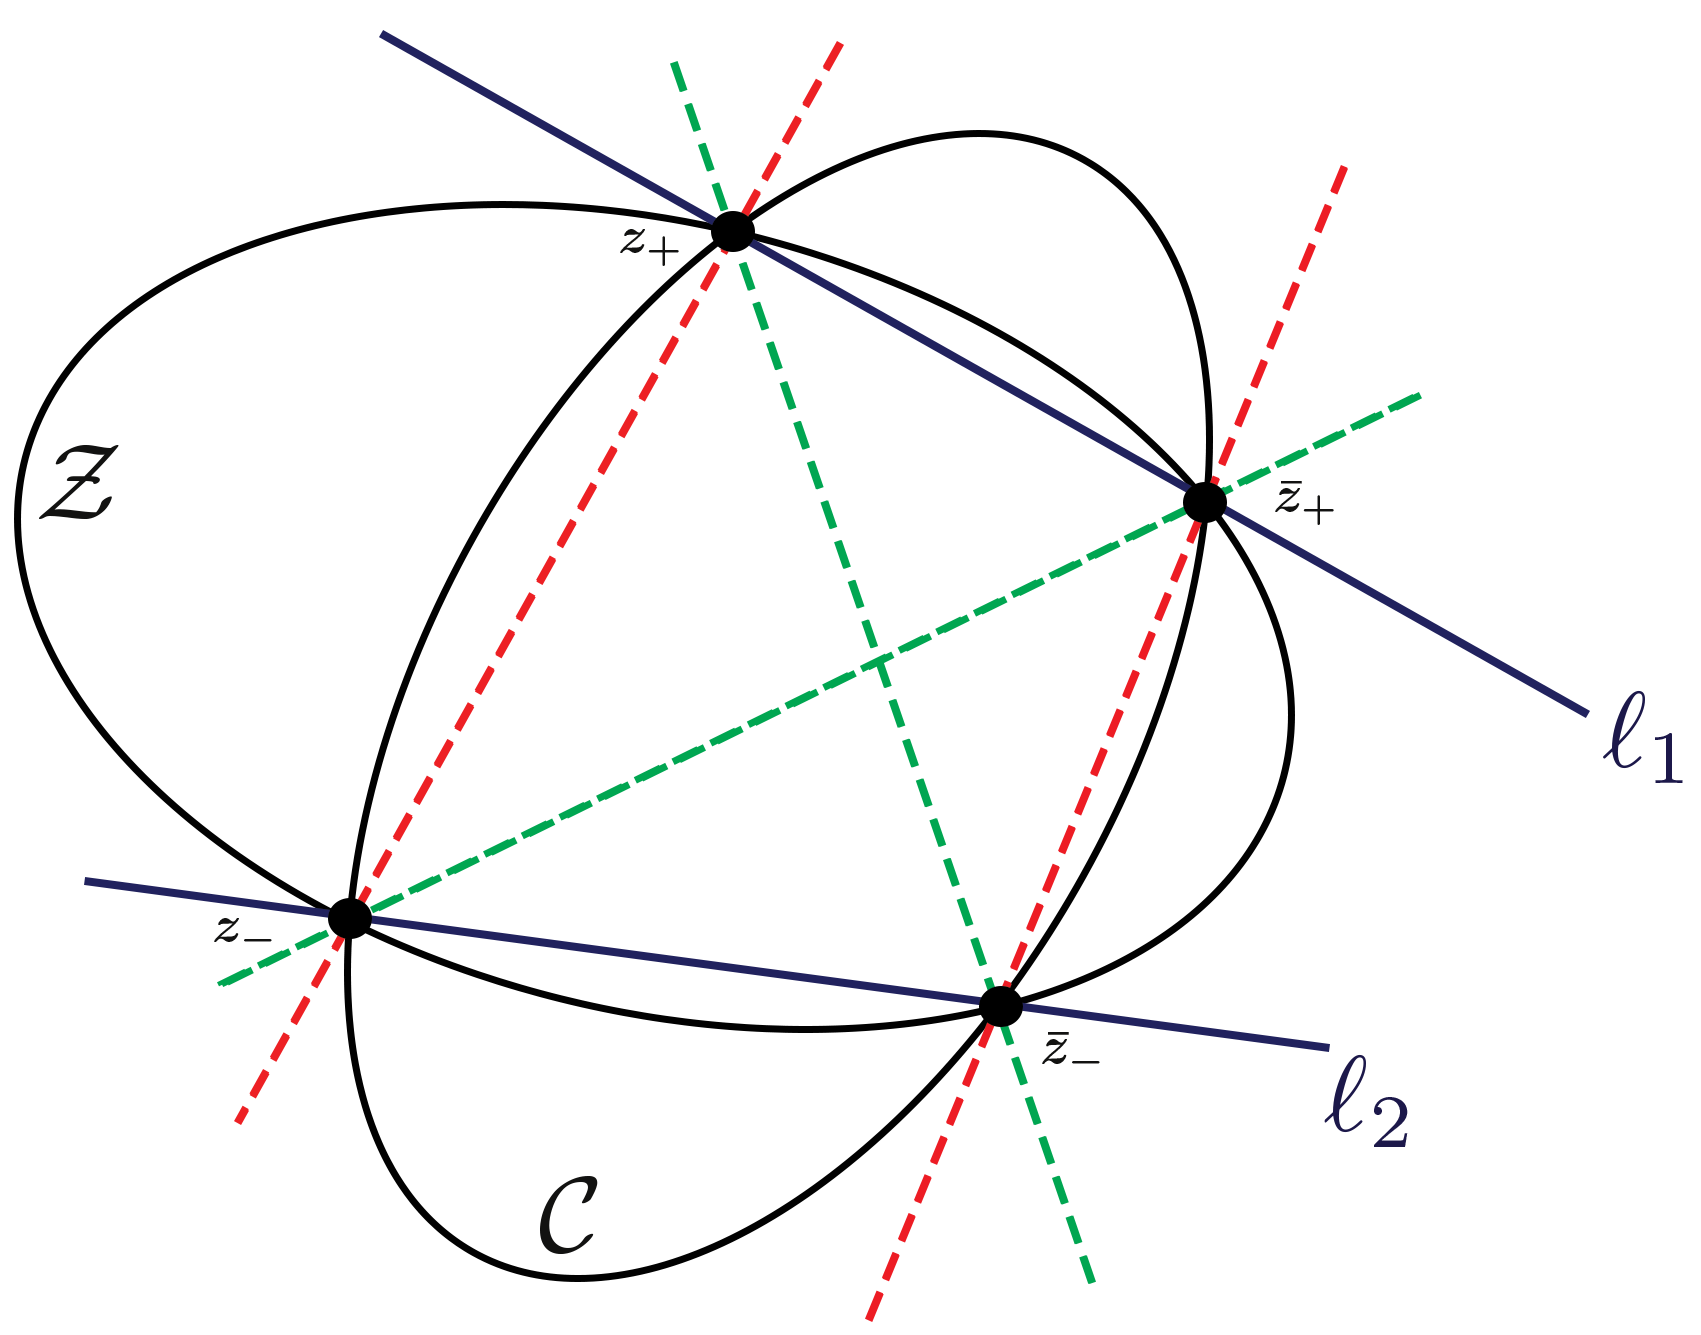
\includegraphics[width=0.6\textwidth]{conics-through-four-points.png}
    \caption[Four intersection points with the absolute conic at infinity.]{Four intersection points of $\mathcal{C}$ and $\mathcal{Z}$ on the plane at infinity, with the imaginary pairs shown in red and green.}
    \label{fig:conics-through-four-points}
\end{figure}

\begin{theorem}
\label{thm:circular-sections-hyperboloid}
Let $Q \subset \mathbb{R}^3$ be the two-sheeted hyperboloid
\begin{equation}
\label{eq:two-sheeted-alpha-beta-gamma}
Q : \frac{x^2}{\alpha} - \frac{y^2}{\beta} - \frac{z^2}{\gamma} = 1
\end{equation}
with $\alpha, \beta, \gamma > 0$ and $\gamma > \beta$. Then the real circular sections of $Q$ are given by the two one-parameter families of parallel planes
\begin{equation}
\label{eq:planes-two-sheeted}
\Pi_{\pm}(\lambda_{\pm}) :\sqrt{\beta (\alpha + \gamma)} x \pm \sqrt{\alpha (\gamma - \beta)} y = \lambda_{\pm}, \quad \quad \lambda_{\pm} \in \mathbb{R} \setminus \left[-\lambda_{0}, \lambda_{0} \right]
\end{equation}
with $\lambda_{0} := \sqrt{\alpha \beta (\alpha+\beta)}$.
\end{theorem}

\begin{proof}
    We embed $\mathbb{R}^3$ into the real projective space $\mathbb{R}\mathbb{P}^3$ and further into the complex projective space $\mathbb{C}\mathbb{P}^3$, and introduce homogeneous coordinates $x_{0}, x_{1}, x_{2}$, and $x_{3}$ such that $x = x_{0} / x_{3}, y = x_{1} / x_{3}$, and $z = x_{2} / x_{3}$. Thus, we identify the plane $x_{3} = 0$ with the plane at infinity. \par
Let $\mathcal{Z}$ denote the absolute conic at infinity (\ref{eq:absolute-conic}), and homogenize the affine equation of $Q$ to get
\[
    \frac{x_{0}^2}{\alpha} - \frac{x_{1}^2}{\beta} - \frac{x_{2}^2}{\gamma} - x_{3}^2 = 0.
\]
Computing the intersection $Q \cap \mathcal{Z}$, we get four points at infinity in the form of two complex-conjugate solutions to the intersecting equations
\[
P_{\pm} =
\begin{bmatrix}[1.5]
\pm \sqrt{\frac{1}{\beta} - \frac{1}{\gamma}}\\
\sqrt{\frac{1}{\alpha} + \frac{1}{\gamma}}\\
i\sqrt{\frac{1}{\alpha} + \frac{1}{\beta}}\\
0
\end{bmatrix},
\quad \text{and} \quad
\overbar{P}_{\pm} =
\begin{bmatrix}[1.5]
\pm \sqrt{\frac{1}{\beta} - \frac{1}{\gamma}}\\
\sqrt{\frac{1}{\alpha} + \frac{1}{\gamma}}\\
-i\sqrt{\frac{1}{\alpha} + \frac{1}{\beta}}\\
0
\end{bmatrix}.
\]
Each complex-conjugate pair spans a real line at infinity. Let $\ell_{\pm} := [P_{\pm}] \vee [\overbar{P}_{\pm}]$. Then its Plücker matrix defined as $[P_{\pm} \overbar{P}_{\pm}^{\top}] - [\overbar{P}_{\pm} P_{\pm}^{\top}]$ is given by the matrix:
\begin{align*}
\begin{bmatrix}
0 && 0 && \mp 2 i \sqrt{\frac{1}{\alpha} + \frac{1}{\beta}} \sqrt{\frac{1}{\beta} - \frac{1}{\gamma}} && 0\\
0 && 0 && -2 i \sqrt{\frac{1}{\alpha} + \frac{1}{\beta}} \sqrt{\frac{1}{\alpha} + \frac{1}{\gamma}} && 0\\
\pm 2 i \sqrt{\frac{1}{\alpha} + \frac{1}{\beta}} \sqrt{\frac{1}{\beta} - \frac{1}{\gamma}} && 2 i \sqrt{\frac{1}{\alpha} + \frac{1}{\beta}}\sqrt{ \frac{1}{\alpha} + \frac{1}{\gamma}} && 0 && 0\\
\end{bmatrix}.
\end{align*}
This is a $4 \times 4$ skew-symmetric homogeneous matrix with rank $2$. Its nullspace spans the pencil of planes with the line $\ell_{\pm}$ as its axis. So the equation of the pencil can be written in homogeneous coordinates, after clearing the denominators as

\[
    \Pi_{\pm}(\lambda_{\pm}) : \sqrt{\beta (\alpha + \gamma)} x_{0} \pm \sqrt{\alpha (\gamma - \beta)} x_{1} - \lambda_{\pm} x_{3} = 0,
\]
where $\lambda_{\pm}$ is the free parameter of the pencil. By construction, the intersection of $\Pi_{\pm}(\lambda_{\pm})$ with $Q$ (if non-empty) gives all the real circular sections of $Q$. \par
It remains to show for which values of $\lambda_{\pm}$ the intersection $Q \cap \Pi_{\pm}(\lambda_{\pm})$ is a non-empty intersection. For this purpose, we identify $Q$ with its Gram matrix
\[
Q =
\begin{bmatrix}
1 / \alpha && 0 && 0 && 0 \\
0 && -1 / \beta && 0 && 0 \\
0 && 0 && -1 / \gamma && 0 \\
0 && 0 && 0 && -1
\end{bmatrix},
\]
such that its corresponding quadratic form $q$ is given by $q(v) = v^{\top} Q v$. The planes of the circular sections $\Pi_{\pm}(\lambda_{\pm})$ correspond to the points
\[
p_{\pm}({\lambda_{\pm}}) =
\begin{bmatrix}[1.3]
\sqrt{\beta (\alpha + \gamma)}\\
\pm \sqrt{\alpha (\gamma - \beta)}\\
0\\
-\lambda_{\pm}
\end{bmatrix}
\]
in the dual projective space $(\mathbb{C}\mathbb{P}^3)^{*}$, and their poles with respect to $Q$ have the coordinates $Q^{-1}p_{\pm}({\lambda_{\pm}})$. Thus, $Q \cap \Pi_{\pm}(\lambda_{\pm})$ is a non-empty if and only if
\[
    q(Q^{-1}p_{\pm}({\lambda_{\pm}})) = \alpha \beta (\alpha + \gamma) - \alpha \beta (\beta - \gamma) - \lambda_{\pm}^2 \geq 0
\]
which is satisfed for $\lambda_{\pm} \in \mathbb{R} \setminus \left[-\lambda_0, \lambda_0\right]$ with $\lambda := \sqrt{\alpha \beta (\alpha+\beta)}$.
\end{proof}

\begin{figure}[H]
  \begin{subfigure}[b]{0.5\textwidth}
    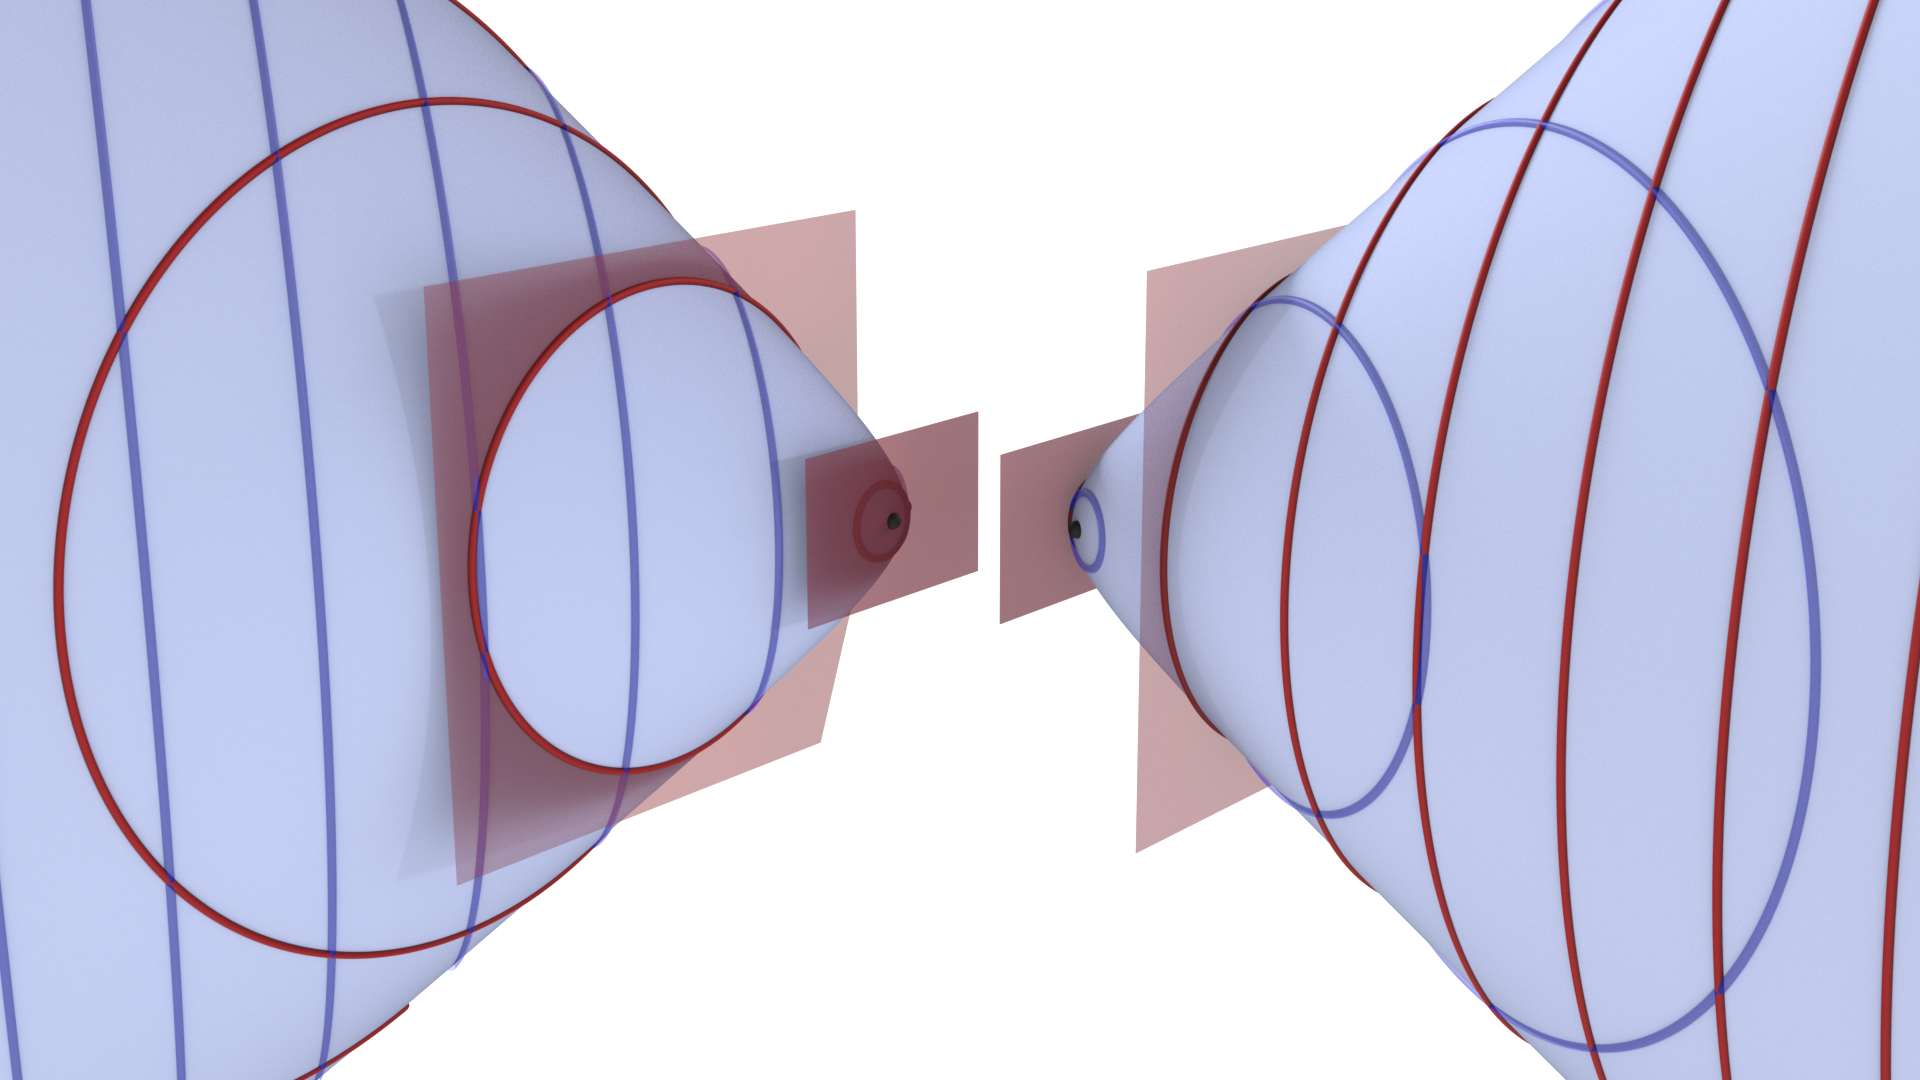
\includegraphics[width=\textwidth]{umbilics_two_sheeted_hyperboloid_red.png}
    \label{fig:two_sheeted_red}
  \end{subfigure}
  \hfill
  \begin{subfigure}[b]{0.5\textwidth}
    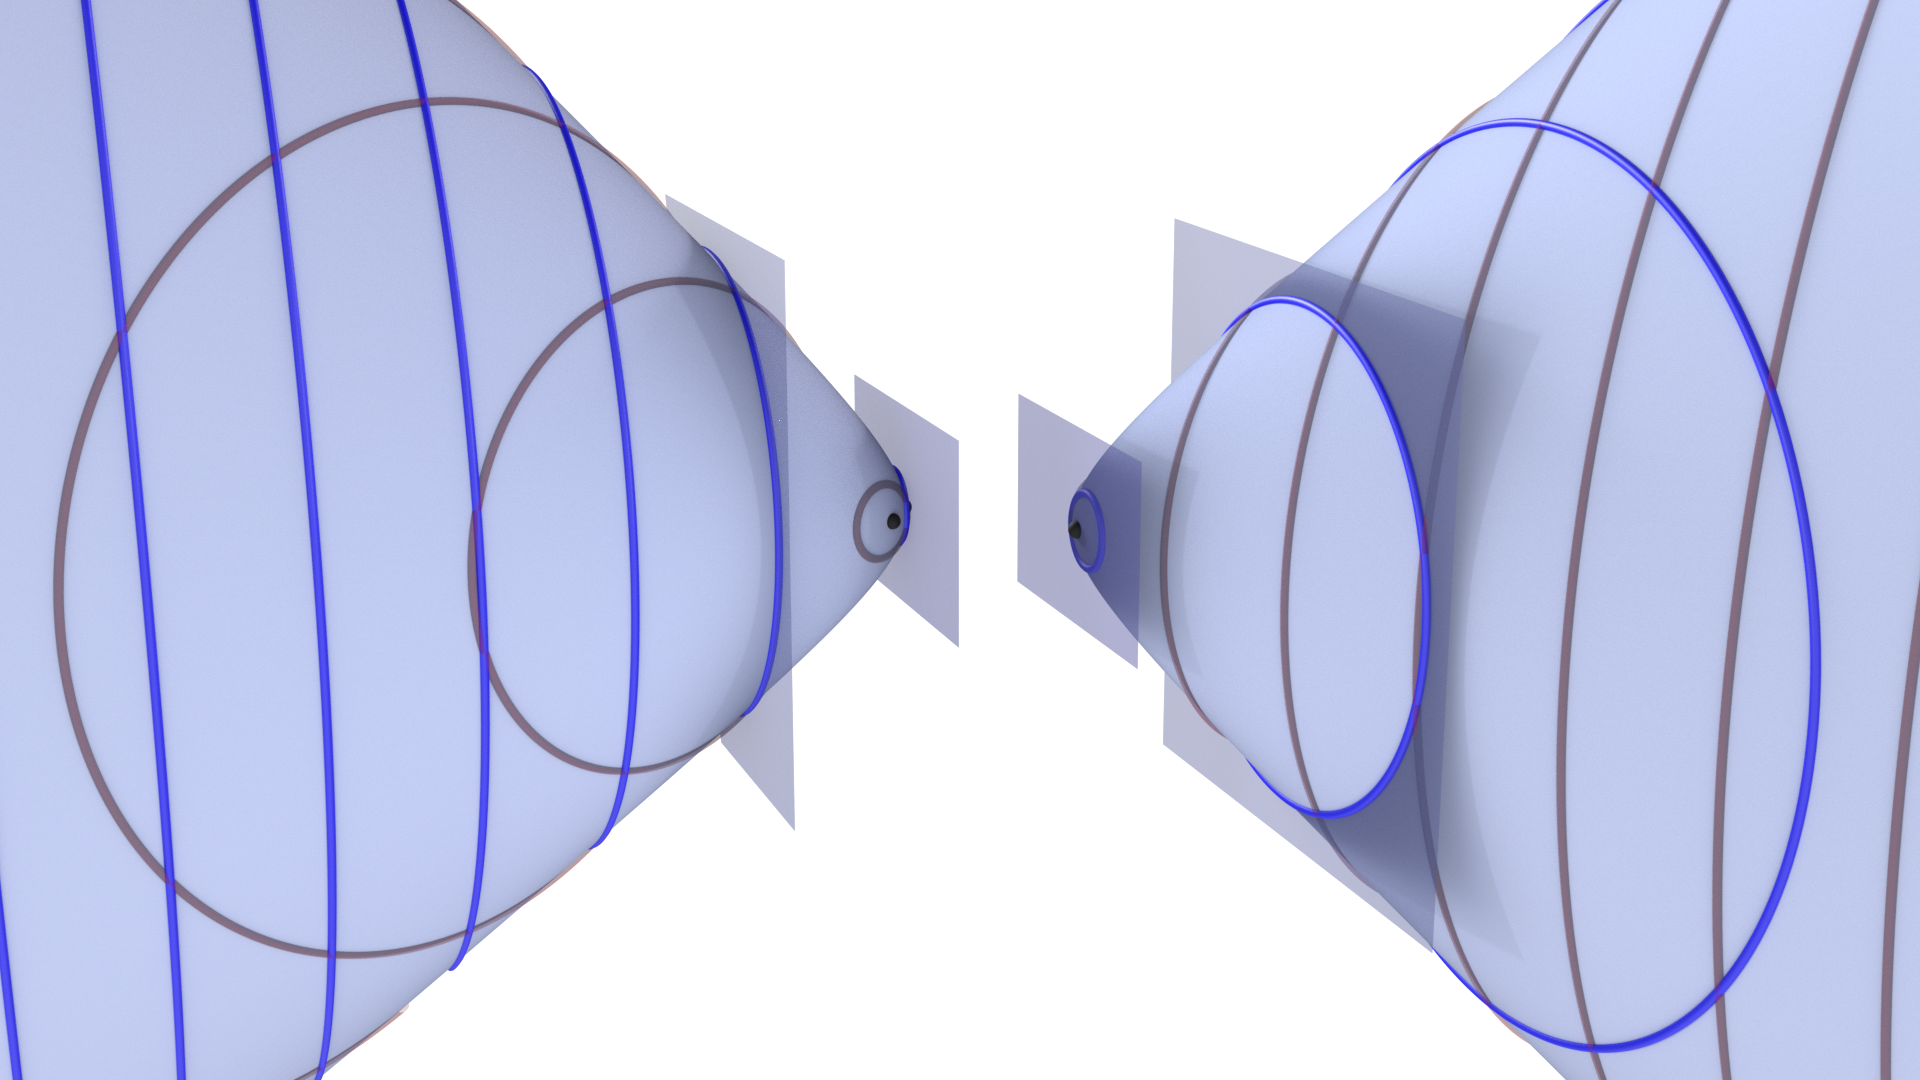
\includegraphics[width=\textwidth]{umbilics_two_sheeted_hyperboloid_blue.png}
    \label{fig:two_sheeted_blue}
  \end{subfigure}
  \caption[Two one-parameter families of circular sections on two-sheeted hyperboloids]{Two-sheeted hyperboloid carry two one-parameter families of circular sections. The planes of circular sections are parallel to the tangent planes at the umbilical points.}
\end{figure}

The same approach employed in the proof of Theorem~\ref{thm:circular-sections-hyperboloid} can be used to explicity compute the circular sections of ellipsoids, one-sheeted hyperboloids, and the elliptical paraboloids. We give the resulting equations here. \par

\begin{itemize}[label=$\blacktriangleright$]
    \item Let $\alpha > \beta > \gamma > 0$, and denote by $\mathcal{E}$ an ellipsoid with equation
        \[
            \mathcal{E} \; : \; \frac{x^2}{\alpha} + \frac{y^2}{\beta} + \frac{z^2}{\gamma} = 1.
        \]
        Then its real circular sections are given by the two families of parallel planes
        \begin{equation}
        \label{eq:planes-ellipsoids}
            \Pi_{\pm}(\lambda_{\pm}) \; : \; \frac{\sqrt{\alpha - \beta}}{\sqrt{\alpha \beta}} x \pm \frac{\sqrt{\beta - \gamma}}{\sqrt{ \beta \gamma}} z = \lambda_{\pm} \quad \quad \lambda_{\pm} \in \left[ -\lambda_{0}, \lambda_{0} \right],
        \end{equation}
        with $\lambda_{0} := \sqrt{\nicefrac{\left(\alpha - \gamma\right)}{\beta}}$. Furthermore, each family of planes is parallel to one of the tangent planes of $\mathcal{E}$ at its umbilical points  \cite{geometryIII}.
    \item Let $\alpha, \beta, \gamma > 0$ with $\alpha > \beta$, and denote by $\mathcal{H}$ a one-sheeted hyperboloid with equation
        \[
            \mathcal{H} \; : \; \frac{x^2}{\alpha} + \frac{y^2}{\beta} - \frac{z^2}{\gamma} = 1.
        \]
        Then its real circular sections are given by the two families of parallel planes
        \begin{equation}
        \label{eq:planes-one-sheeted}
            \Pi_{\pm}(\lambda_{\pm}) \; : \;  \sqrt{ \gamma (\alpha- \beta) } \ y \pm \sqrt{\beta(\alpha+\gamma)} \ z = \pm \; \lambda_{\pm} \quad \quad \lambda_{\pm} \in \mathbb{R}.
        \end{equation}
    \item Let $\alpha > \beta > 0$, and denote by $\mathcal{P}$ an elliptical paraboloid with equation
        \[
            \mathcal{P} \; : \; \frac{x^2}{\alpha} + \frac{y^2}{\beta} - 2 z = 0.
        \]
        Then its circular sections are given by the two families of parallel planes
        \begin{equation}
        \label{eq:planes-paraboloids}
            \Pi_{\pm}(\lambda_{\pm}) \; : \; \frac{\sqrt{\alpha - \beta}}{\sqrt{\alpha \beta}} y \pm \frac{1}{\sqrt{\alpha}} z = \lambda_{\pm}.
        \end{equation}
        As in the case of ellipsoids and two-sheeted hyperboloids, the planes are parallel to the tangent planes of $\mathcal{P}$ at its umbilical points.
\end{itemize}

\sloppy For a complementary perspective on circles on quadrics, one can refer to \cite{nilovSurfaceContainingLine2011}, in particular \cite[\textcolor{CitationColor}{Lemma~2.1.}]{nilovSurfaceContainingLine2011}, and \cite[\textcolor{CitationColor}{Lemma~2.6}]{nilovSurfaceContainingLine2011}.

\begin{figure}[H]
    \centering
    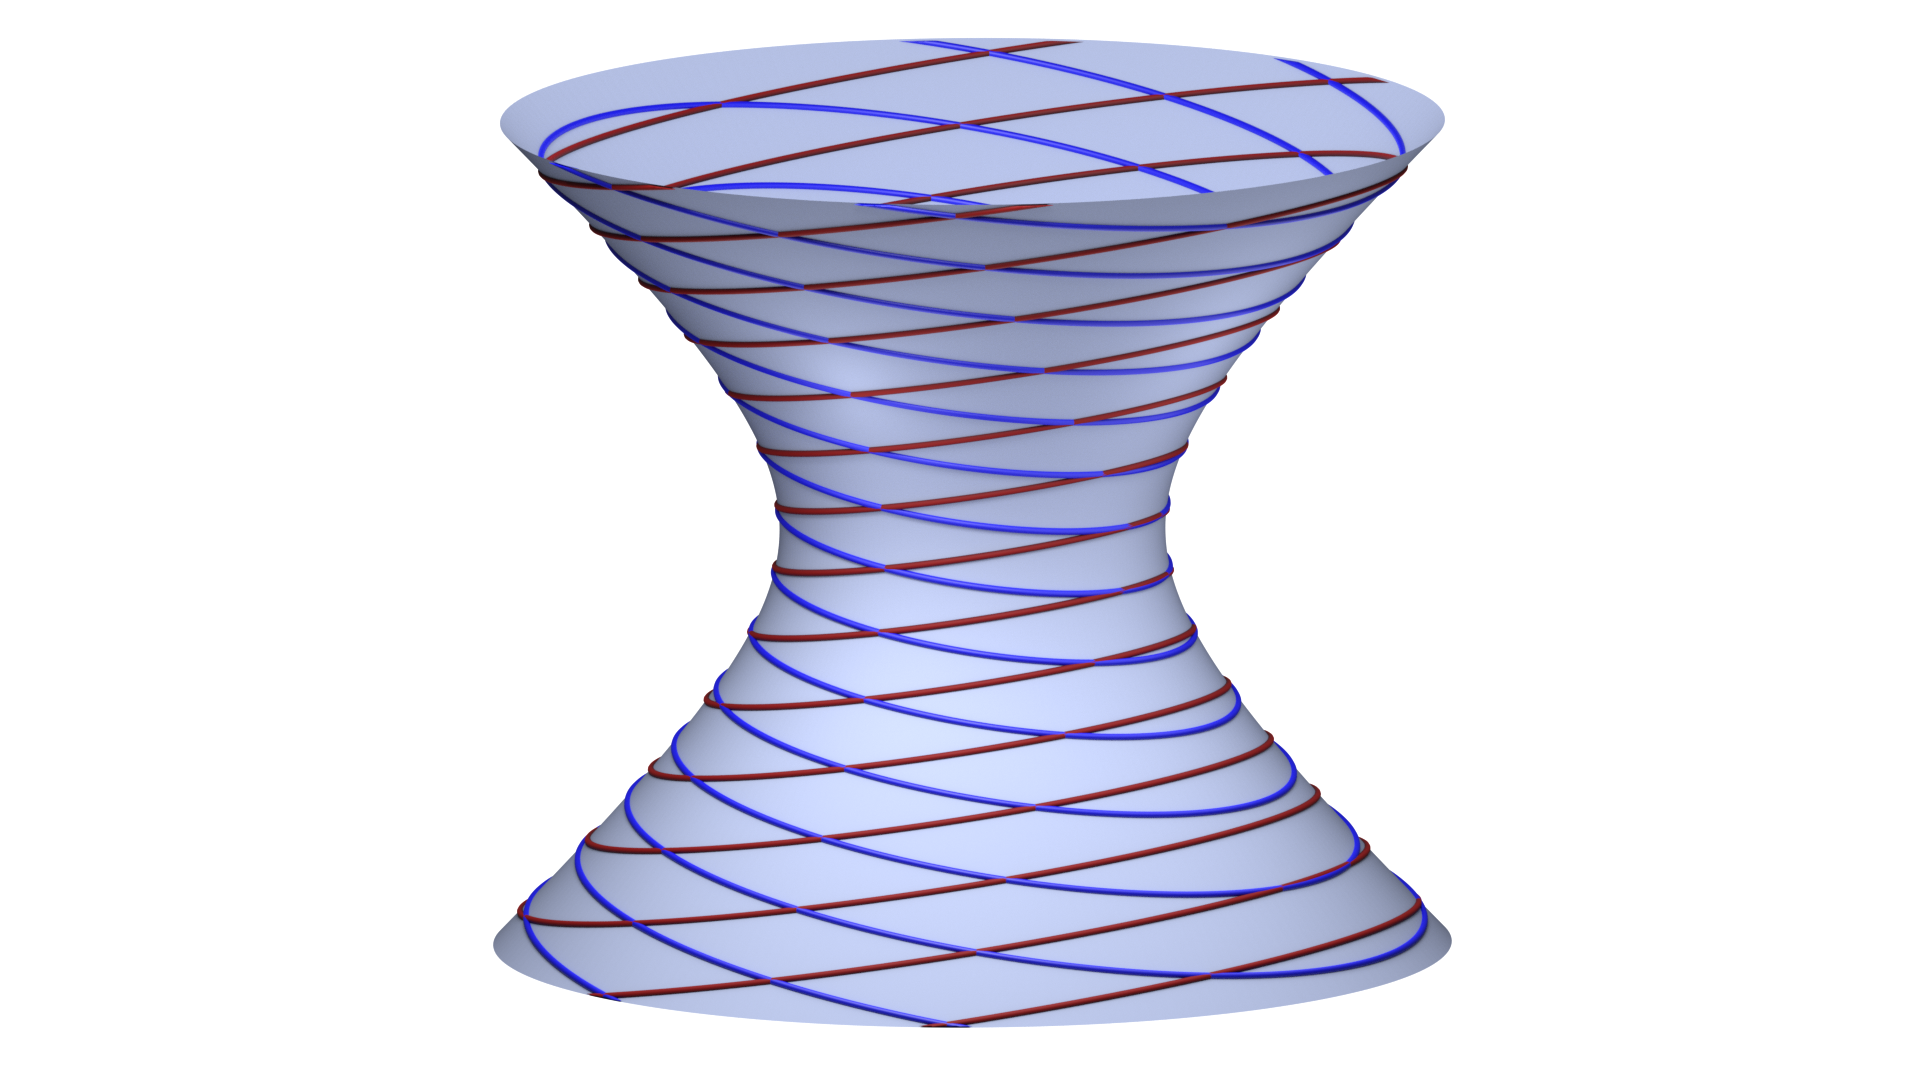
\includegraphics[width=0.7\textwidth]{circles_sections_of_one_sheeted_hyperboloid.png}
    \caption{One-sheeted hyperboloids carry two one-parameter families of circular sections.}
    \label{fig:circular_sections_one_sheeted}
\end{figure}

\pagebreak
%===========================================================
\section{Families of confocal quadrics}
\label{sec:confocal-quadrics}

\begin{definition}
\label{def:confocal-quadrics}
In Euclidean geometry, two quadrics in $\mathbb{R}^3$ are \textit{confocal}, sometimes also referred to as \textit{homofocal}, if they have common axes and intersect each plane of symmetry along confocal conics.
\end{definition}

Non-degenerate families of confocal quadrics come in two types:
\begin{itemize}[label=$\blacktriangleright$]
    \item Ellipsoids, hyperboloids of one sheet, and hyperboloids of two sheets,
    \item Downward-pointing elliptical paraboloids, upward-pointing elliptic paraboloids, and hyperbolic paraboloids.
\end{itemize}
For the remainder of this thesis, the term \textit{confocal quadrics} will refer only to the first type, i.e. a family of confocal ellipsoids, hyperboloids of one sheet, and hyperboloids of two sheets. \par

\begin{proposition}
\label{prop:normal-form}
Any ellipsoid, one-sheeted hyperboloid, or two-sheeted hyperboloid $\mathbb{R}^3$ can be brought into the following normal form by a Euclidean motion $\boldsymbol{x} \mapsto A \boldsymbol{x} + \boldsymbol{b}$:
\[
    \mathcal{Q} \; : \; \frac{x^2}{a} + \frac{y^2}{b} + \frac{z^2}{c} = 1
\]
for some $a > 0$, $b, c \neq 0$, and $a > b > c$.
\end{proposition}

\begin{proof}
    See \cite[\textcolor{CitationColor}{Ch.~3}]{odehnalUniverseQuadrics2020}.
\end{proof}

Let $a, b, c \in \mathbb{R}$ with $a > b > c$ and consider a non-degenerate, non-parabolic quadric in normal form
\[
    \frac{x^2}{a} + \frac{y^2}{b} + \frac{z^2}{c} = 1.
\]
Then any quadric confocal with it must necessarily be in normal form
\[
    \frac{x^2}{\tilde{a}} + \frac{y^2}{\tilde{b}} + \frac{z^2}{\tilde{c}} = 1
\]
with $\tilde{a} > \tilde{b} > \tilde{c}$, and the differences between the fixed parameters of each quadric must all be equal, i.e.
\[
    a - b = \tilde{a} - \tilde{b}, \quad a - c = \tilde{a} - \tilde{c}, \ \text{ and } \  b - c = \tilde{b} - \tilde{c}.
\]
This motivates the following definition \cite{geometryIII}:

\begin{definition}[]
\label{def:family-of-confocal-quadrics}
Let $a, b, c \in \mathbb{R}$ with $a > b > c > 0$. The one-parameter family of quadrics given by
\[
    Q_{\lambda} := \left\{ (x, y, z) \in \mathbb{R}^3 : \frac{x^2}{a + \lambda} + \frac{y^2}{b + \lambda} + \frac{z^2}{c + \lambda} = 1 \right\}, \quad \lambda \in \mathbb{R}
\]
is called a family of \textit{confocal quadrics}.
\end{definition}

Any triple of real numbers $a, b$, and $c$ divides the real line into four segments, and we can recover the subfamilies of quadrics of different signatures in the confocal family accordingly:

\begin{itemize}[label=$\blacktriangleright$]
    \item If $\lambda < -a$, then $Q_{\lambda}$ is purely imaginary with no real points.
    \item If $\lambda \in (-a, -b)$, then $Q_{\lambda}$ is a one-parameter family of confocal two-sheeted hyperboloids.
    \item If $\lambda \in (-b, -c)$, then $Q_{\lambda}$ is a one-parameter family of confocal one-sheeted hyperboloids.
    \item If $\lambda > -c$, then $Q_{\lambda}$ is a one-parameter family of confocal ellipsoids. \par
\end{itemize}

\begin{theorem}[]
\label{thm:fill-up-euclidean-space}
For every point $(x, y, z) \in \mathbb{R}^3$ with $x \cdot y \cdot z \neq 0$, i.e. a point not on the standard coordinate planes, there passes exactly one ellipsoid, one one-sheeted hyperboloid, and one two-sheeted hyperboloid from the confocal family $Q_{\lambda}$.
\end{theorem}

\begin{proof}
    Let $a, b, c \in \mathbb{R}$ be the fixed parameters of the confocal family
\begin{equation}
\label{eq:confocal-family-fixed-point}
    Q_{\lambda} \; : \; \frac{x^2}{a + \lambda} + \frac{y^2}{b + \lambda} + \frac{z^2}{c + \lambda} = 1,
\end{equation}
with $a > b > c > 0$. Given any point $(x, y, z) \in \mathbb{R}^3$, and after clearing the denominators of equation (\ref{eq:confocal-family-fixed-point}), we can see that it's a third degree polynomial equation in $\lambda$. Thus, it has three roots $u_{1}, u_{2}$, and $u_{3}$ which can be solved for explicitly. For our purposes, it's enough to note that these roots are real, and lie in the intervals
\[
    -a < u_{1} < -b < u_{2} < -c < u_{1}
\]
by looking at the qualitative behavior of the function
\[
    \lambda \mapsto \frac{x^2}{a + \lambda} + \frac{y^2}{b + \lambda} + \frac{z^2}{c + \lambda}
\]
over $\mathbb{R}$ [Figure~\ref{fig:plot}].
\end{proof}

\begin{figure}[H]
    \centering
    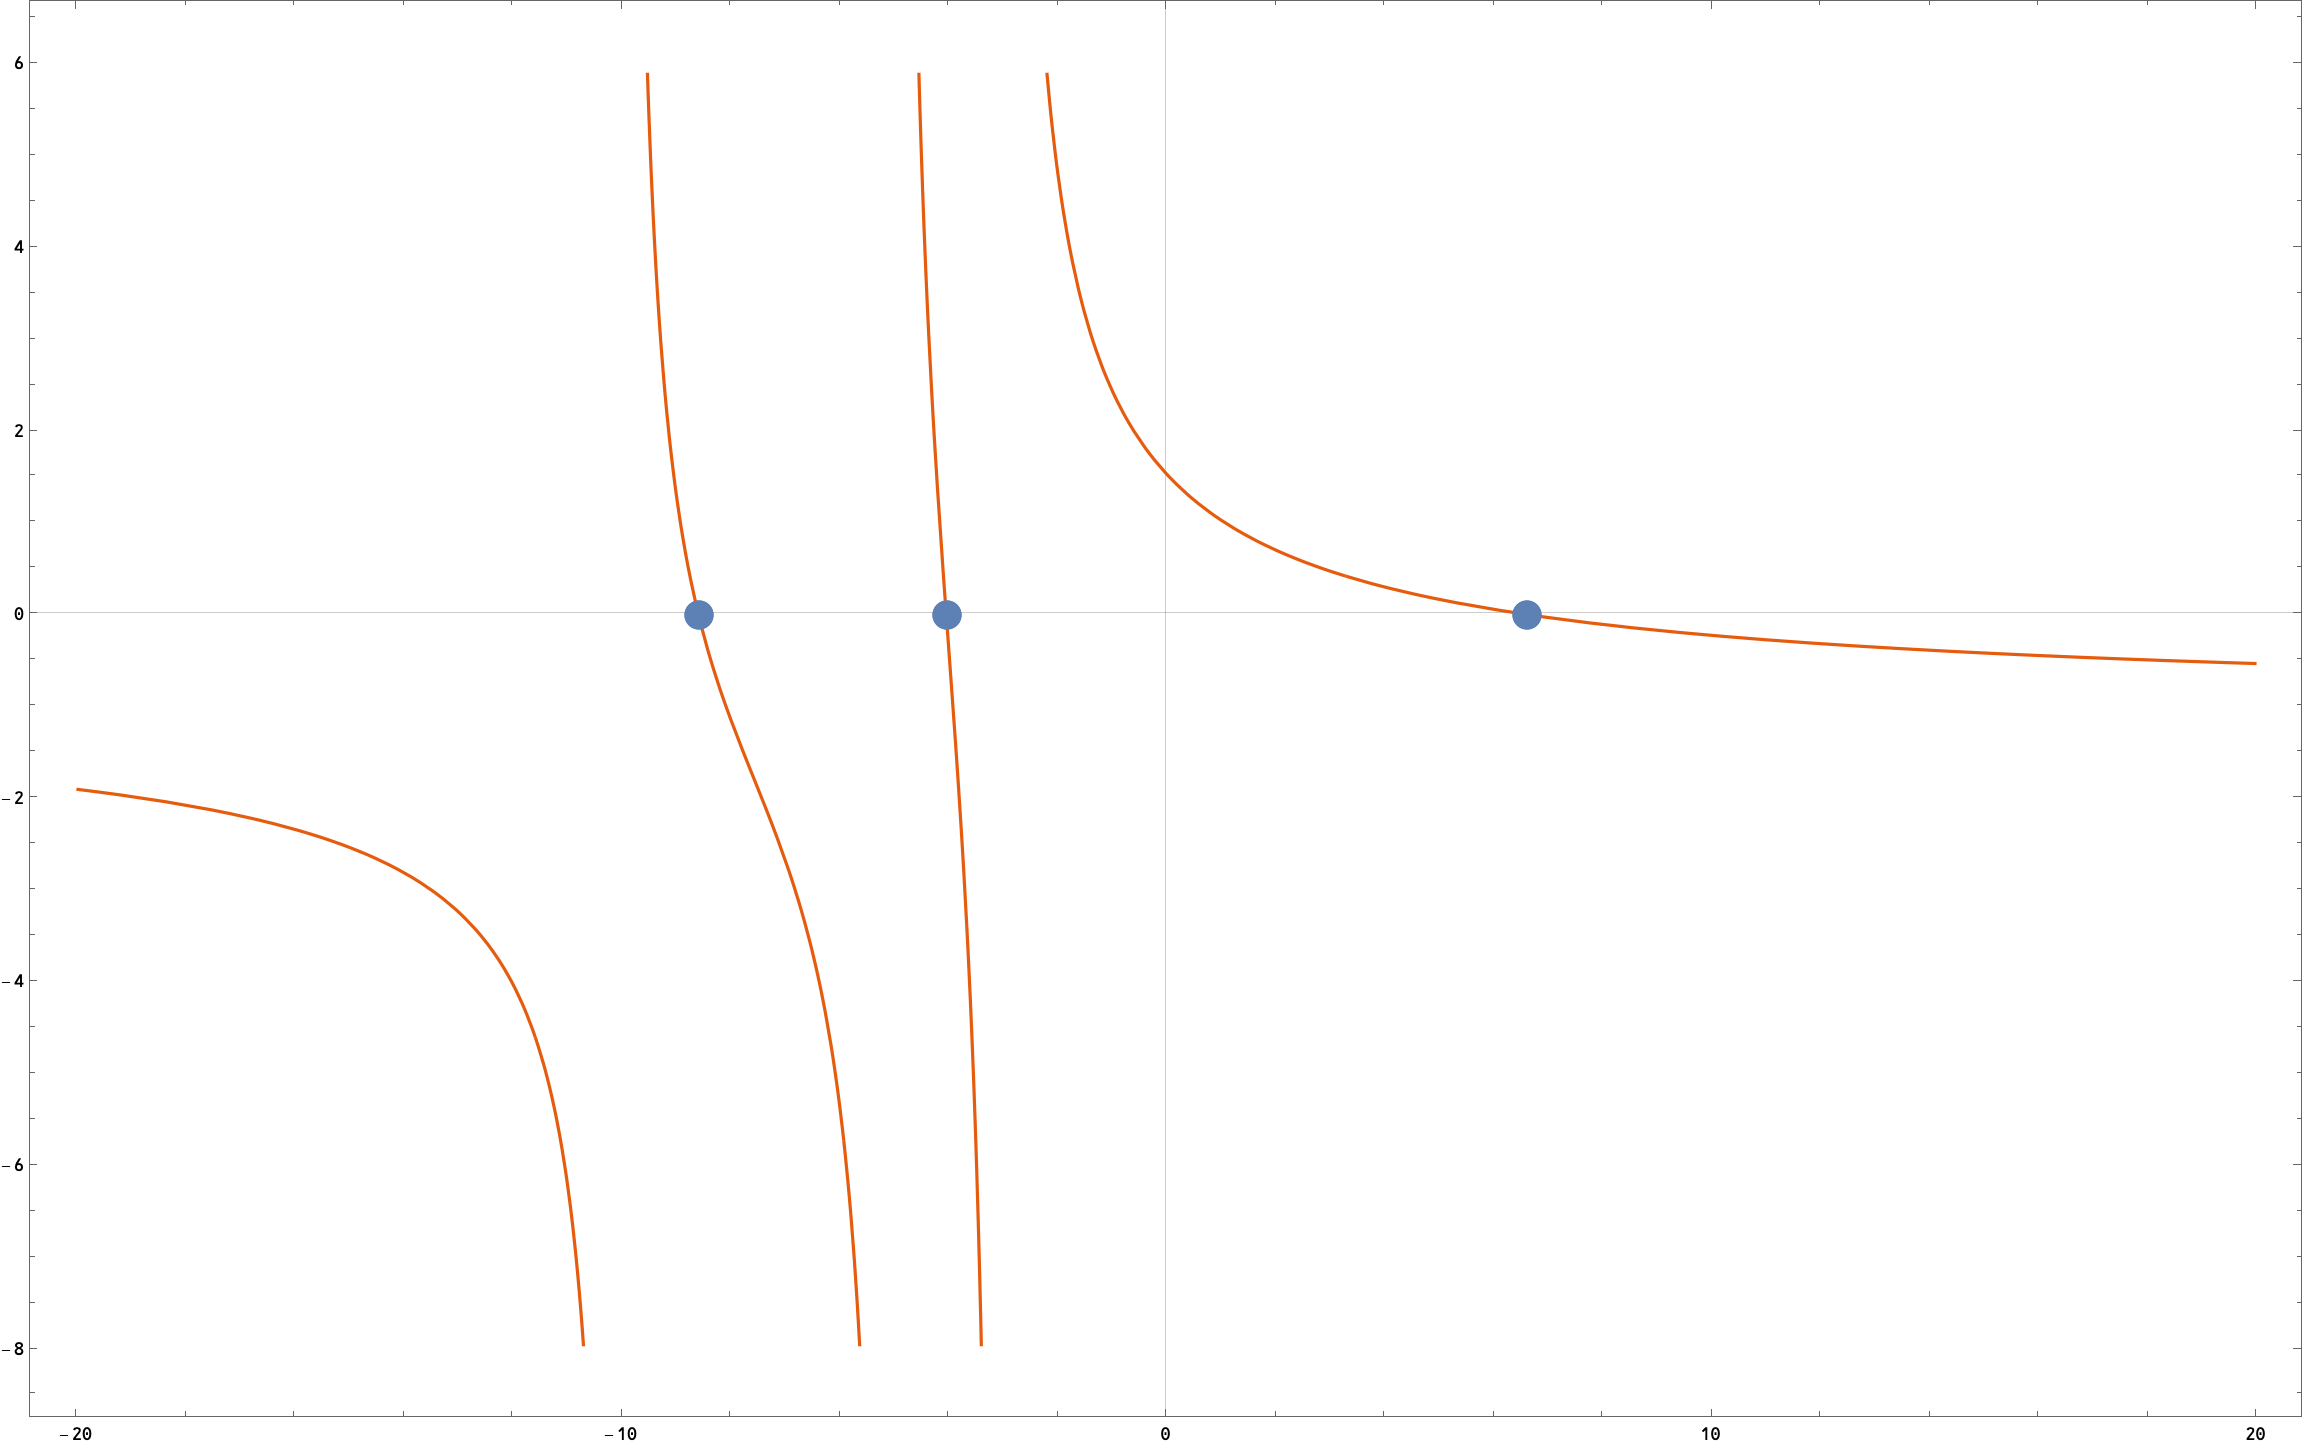
\includegraphics[width=1.0\textwidth]{graph-for-proof.png}
    \label{fig:graph-for-proof}
    \caption[A plot of the real-valued function $\lambda \mapsto \frac{x^2}{a + \lambda} + \frac{y^2}{b + \lambda} + \frac{z^2}{c + \lambda}$]{The function $\lambda \mapsto \frac{x^2}{a + \lambda} + \frac{y^2}{b + \lambda} + \frac{z^2}{c + \lambda}$ plotted for some $(x_0, y_0, z_0) \in \mathbb{R}^3$, $a = 10.0$, $b = 5.0$, and $c = 3.0$.}
    \label{fig:plot}
\end{figure}

\begin{theorem}
\label{thm:confocal-quadrics-intersect-eight-points}
A confocal ellipsoid, one-sheeted hyperboloid, and two-sheeted hyperboloid intersect orthogonally in eight points in $\mathbb{R}^3$, which lie mirror symmetric with respect to the common principal planes.
\end{theorem}
\begin{proof}
Let $a > b > c > 0$, and define the confocal family
\[
    \mathcal{Q}_{\lambda} \; : \; \frac{x^2}{a + \lambda} + \frac{y^2}{b + \lambda} + \frac{z^2}{c + \lambda} = 1.
\]
Then for any fixed $u_{1}, u_{2}, u_{3} \in \mathbb{R}$ with $-a < u_{1} < -b < u_{2} < -c < u_{3}$, the quadrics
\begin{equation}
\label{eq:the-quadrics-u1u2u3}
\begin{aligned}
\mathcal{Q}_{u_{1}} \; : \; \frac{x^2}{u_{1} + a} + \frac{y^2}{u_{1} + b} + \frac{z^2}{u_{1} + c} &= 1 \\
\mathcal{Q}_{u_{2}}\; : \; \frac{x^2}{u_{2} + a} + \frac{y^2}{u_{2} + b} + \frac{z^2}{u_{2} + c} &= 1 \\
\mathcal{Q}_{u_{3}} \; : \; \frac{x^2}{u_{3} + a} + \frac{y^2}{u_{3} + b} + \frac{z^2}{u_{3} + c} &= 1
\end{aligned}
\end{equation}
respectively determine a confocal two-sheeted hyperboloid, one-sheeted hyperboloid, and ellipsoid. \par
Define $g : \mathbb{R} \to \mathbb{R}$ such that
\[
    g(\lambda) = \frac{x^2}{a + \lambda} + \frac{y^2}{b + \lambda} + \frac{z^2}{c + \lambda} - 1.
\]
Then $g$ has three first-order poles at $\lambda = -a, \lambda = -b$, and $\lambda = -c$. So we can compute its residues by
\begin{align*}
\underset{\lambda = -a}{\text{res}} g(\lambda) &= \lim_{\lambda \to -a} (\lambda + a) g(\lambda) \\
&= \lim_{\lambda \to -a} x^2 + \frac{\lambda + a}{\lambda + b}  y^2 + \frac{\lambda + a}{\lambda + c} z^2 - (\lambda + a) = x^2.
\end{align*}
Similarly, $\text{res}_{\lambda = -b} g(\lambda) = y^2$, and $\text{res}_{\lambda = -c} g(\lambda) = z^2$. Consider the third-degree polynomial in $\lambda$ given by
\begin{align*}
p(\lambda) &:= (a+\lambda)(b+\lambda)(c+\lambda)g(\lambda) \\
&\;= (b+\lambda)(c+\lambda)x^2 + (a+\lambda)(c+\lambda)y^2 + (a+\lambda)(b+\lambda)z^2  - (a+\lambda)(b+\lambda)(c+\lambda),
\end{align*}
with its highest order coefficient equal to $-1$. Since $g(u_{1}) = g(u_{2}) = g(u_{3}) = 0$, it follows that $p$ has three distinct real roots at $\lambda = u_{1}, \lambda = u_{2}$, and $\lambda = u_{3}$. Thus, we can factorize it as
\[
    p(\lambda) = -(\lambda - u_{1})(\lambda - u_{2})(\lambda - u_{3}).
\]
This yields the following form for $g$
\begin{align*}
g(\lambda) &= \frac{-(\lambda - u_{1})(\lambda - u_{2})(\lambda - u_{3})}{(a+\lambda)(b+\lambda)(c+\lambda)},
\end{align*}
which can be used to re-compute its residues:
\begin{align*}
\underset{\lambda = -a}{\text{res}} g(\lambda) &= \lim_{\lambda \to -a} (\lambda + a)g(\lambda) \\
&= \lim_{\lambda \to -a} \frac{-(\lambda - u_{1})(\lambda - u_{2})(\lambda - u_{3})}{(b+\lambda)(c+\lambda)} \\
&= \frac{(u_{1} + a)(u_{2} + a)(u_{3} + a)}{(a-b)(a-c)},
\end{align*}
and similarly,
\begin{align*}
\underset{\lambda = -b}{\text{res}} g(\lambda) &= \frac{(u_{1} + b)(u_{2} + b)(u_{3} + b)}{(a-b)(c-b)}, \\
\underset{\lambda = -c}{\text{res}} g(\lambda) &= \frac{(u_{1} + c)(u_{2} + c)(u_{3} + c)}{(a-c)(b-c)}.
\end{align*}
Equating both results, we get the following:
\begin{equation}
\label{eq:squared-xyz-form}
\begin{aligned}
x^2 &= \frac{(u_{1} + a)(u_{2} + a)(u_{3} + a)}{(a-b)(a-c)} \\
y^2 &= \frac{(u_{1} + b)(u_{2} + b)(u_{3} + b)}{(a-b)(c-b)} \\
z^2 &= \frac{(u_{1} + c)(u_{2} + c)(u_{3} + c)}{(a-c)(b-c)}.
\end{aligned}
\end{equation}
Since the right-hand side of all equations is positive, there exists eight solutions for $(x, y, z)$ given by
\begin{equation}
\label{eq:sqrt-root-parameterization}
\begin{aligned}
x &= \pm \frac{\sqrt{u_{1} + a}\sqrt{u_{2} + a}\sqrt{u_{3} + a }}{\sqrt{a-b}\sqrt{a-c}} \\
y &= \pm \frac{\sqrt{-(u_{1} + b)}\sqrt{u_{2} + b}\sqrt{u_{3} + b}}{\sqrt{a-b}\sqrt{b-c}} \\
z &= \pm \frac{\sqrt{-(u_{1} + c)}\sqrt{-(u_{2} + c)}\sqrt{u_{3} + c}}{\sqrt{a-c}\sqrt{b-c}}
\end{aligned}
\end{equation}
Each solution is contained in one octant of $\mathbb{R}^3$, mirror symmetric with respect to the common principal planes. \par
It remains to show that the confocal quadrics intersect orthogonally. Define a one-parameter family of functions
\[
    f_{\lambda} : \mathbb{R}^3 \to \mathbb{R}, \quad \quad (x, y, z) \mapsto \frac{x^2}{a + \lambda} + \frac{y^2}{b + \lambda} + \frac{z^2}{c + \lambda}.
\]
Then the confocal quadrics can be defined as level sets of $f_{\lambda}$, i.e. $\mathcal{Q}_{\lambda} = f^{-1}_{\lambda}(\{1\})$. The gradient of $f_{\lambda}$ is given by
\[
    \text{grad} \; f_{\lambda}(x, y, z) = \left( \frac{2x}{a + \lambda}, \frac{2y}{b + \lambda}, \frac{2z}{c + \lambda} \right).
\]
Let $(x, y, z) \in \mathbb{R}^3$ be one of the eight intersection points of the corresponding confocal quadrics, i.e. $(x, y, z) \in \mathcal{Q}_{u_{1}} \cap \mathcal{Q}_{u_{3}} \cap \mathcal{Q}_{u_{3}}$. To show that the quadrics intersect orthogonally, we just need to show that the gradients, which span the normal lines to the quadrics at their intersection points, are orthogonal. We have
\begin{align*}
\left< \text{grad} \; f_{u_{1}}(x, y, z), \text{grad} \; f_{u_{2}}(x, y, z)  \right> &= \left< \left( \frac{2x}{a + u_{1}}, \frac{2y}{b + u_{1}}, \frac{2z}{c + u_{1}} \right), \left( \frac{2x}{a + u_{2}}, \frac{2y}{b + u_{2}}, \frac{2z}{c + u_{2}} \right) \right>  \\
&= 4 \left( \frac{x^2}{(a + u_{1})(a + u_{2})} + \frac{y^2}{(b + u_{1})(b + u_{2})} + \frac{z^2}{(c + u_{1})(c + u_{2})} \right) \\
&= 4 \left( \frac{u_{3} + a}{(a - b)(a - c)} - \frac{u_{3} + b}{(a - b)(b - c)} + \frac{u_{3} + c}{(a - c)(b - c)} \right) = 0.
\end{align*}
where the last equality follows from (\ref{eq:squared-xyz-form}), and similarly $\left< \text{grad} \; f_{u_{1}}(x, y, z), \text{grad} \; f_{u_{3}}(x, y, z)  \right> = 0$, and $\left< \text{grad} \; f_{u_{2}}(x, y, z), \text{grad} \; f_{u_{3}}(x, y, z)  \right> = 0$.
\end{proof}

\subsection{Confocal Coordinates}
\label{subsec:confocal-coordinates}
In Theorem~\ref{thm:fill-up-euclidean-space}, we have shown that every point $(x, y, z) \in \mathbb{R}^3$ with $x \cdot y \cdot z \neq 0$ is the intersection of three confocal quadrics. Conversely, as stated in Theorem~\ref{thm:confocal-quadrics-intersect-eight-points}
, every triple of confocal quadrics with distinct signatures meet orthogonally in a unique point $(x, y, z)$ in each octant of $\mathbb{R}^3$. Thus, any triple of real numbers $a, b$, and $c$ with $a > b > c$ determines a \textit{triply orthogonal coordinate system} derived naturally from confocal quadrics. For example, the map
\[
\boldsymbol{x} :  \mathcal{U} \to \mathbb{R}_{+}^3, \quad \quad \boldsymbol{x}(s_{1}, s_{2}, s_{3}) \mapsto \begin{pmatrix}
x(s_{1}, s_{2}, s_{3}) \\
y(s_{1}, s_{2}, s_{3}) \\
z(s_{1}, s_{2}, s_{3})
\end{pmatrix}
\]
with $\mathcal{U} := \{ (u_{1}, u_{2}, u_{3}) \in \mathbb{R}^3 \; : \; -a < u_{1} < -b < u_{2} < -c < u_{3}\}$, and
\begin{align*}
x &= \frac{\sqrt{u_{1} + a}\sqrt{u_{2} + a}\sqrt{u_{3} + a }}{\sqrt{a-b}\sqrt{a-c}}, \\
y &= \frac{\sqrt{-(u_{1} + b)}\sqrt{u_{2} + b}\sqrt{u_{3} + b}}{\sqrt{a-b}\sqrt{b-c}}, \\
z &= \frac{\sqrt{-(u_{1} + c)}\sqrt{-(u_{2} + c)}\sqrt{u_{3} + c}}{\sqrt{a-c}\sqrt{b-c}}.
\end{align*}
parameterizes the octant $\mathbb{R}_{+}^3 := \{ (x, y, z)\in \mathbb{R}^3 \; : \; x > 0, y > 0, z > 0 \}$.

\begin{definition}
\label{def:confocal-coordinates}
A coordinate system $\boldsymbol{x} : \mathbb{R}^3 \to \mathbb{R}^3$ is called a \textit{confocal coordinate system}, if its coordinate surfaces $\boldsymbol{x}(u_{1}=\text{const.}, u_{2}, u_{3})$, $\boldsymbol{x}(u_{1}, u_{2}=\text{const.}, u_{3})$, and $\boldsymbol{x}(u_{1}, u_{2}, u_{3}=\text{const.})$ are contained in confocal quadrics.
\end{definition}

It's often useful to reparameterize the coordinate lines of a confocal system according to $u_{i} = u_{i}(s_{i})$. This allows us to obtain new representations of the same system with particularly nice properties.

\begin{theorem}
\label{thm:main-confocal-system}
Let
\[
\boldsymbol{x} : I_{1} \times I_{2} \times I_{3} \subset \mathbb{R}^3 \to \mathbb{R}^3, \quad \quad \boldsymbol{x}(s_{1}, s_{2}, s_{3}) \mapsto \begin{pmatrix}
x(s_{1}, s_{2}, s_{3}) \\
y(s_{1}, s_{2}, s_{3}) \\
z(s_{1}, s_{2}, s_{3})
\end{pmatrix}
\]
be a coordinate system. Then $\boldsymbol{x}$ is a confocal coordinate system if and only if it can be written in the form
\begin{equation}
\begin{aligned}
\label{eq:main-parameterization}
x(s_{1}, s_{2}, s_{3}) &= \frac{f_{1}(s_{1}) f_{2}(s_{2}) f_{3}(s_{3})}{\sqrt{(a - b) (a - c)}} \\
y(s_{1}, s_{2}, s_{3}) &= \frac{g_{1}(s_{1}) g_{2}(s_{2}) g_{3}(s_{3})}{\sqrt{(a - b) (b - c)}} \\
z(s_{1}, s_{2}, s_{3}) &= \frac{h_{1}(s_{1}) h_{2}(s_{2}) h_{3}(s_{3})}{\sqrt{(a - c) (b - c)}}
\end{aligned}
\end{equation}
where the functions $f_{i}, g_{i}$, and $h_{i}$ are real-valued functions of a single variable
\[
f_{1}, g_{1}, h_{1} : I_{1} \to \mathbb{R}, \quad f_{2}, g_{2}, h_{2} : I_{2} \to \mathbb{R}, \quad \text{and} \quad f_{3}, g_{3}, h_{3} : I_{3} \to \mathbb{R}
\]
related by the functional equations
\begin{equation}
\begin{aligned}
\label{eq:functional-relations}
f_{1}(s_{1})^2 + g_{1}(s_{1})^2 &= a - b, \quad f_{1}(s_{1})^2 + h_{1}(s_{1})^2 = a - c \\
f_{2}(s_{2})^2 - g_{2}(s_{2})^2 &= a - b, \quad f_{2}(s_{2})^2 + h_{2}(s_{2})^2 = a - c \\
f_{3}(s_{3})^2 - g_{3}(s_{3})^2 &= a - b, \quad f_{3}(s_{3})^2 - h_{3}(s_{3})^2 = a - c
\end{aligned}
\end{equation}
\end{theorem}

\begin{proof}
Let $\boldsymbol{x}$ be a confocal coordinate system. Then there exist $a, b, c \in \mathbb{R}$ with $a > b > c$, and smooth functions
\begin{equation*}
\begin{aligned}
u_{1} : I_{1} \to \mathcal{I}_{1}, &\quad \quad s_{1} \mapsto u_{1}(s_{1}) \\
u_{2} : I_{2} \to \mathcal{I}_{2}, &\quad \quad s_{2} \mapsto u_{2}(s_{2}) \\
u_{2} : I_{3} \to \mathcal{I}_{3}, &\quad \quad s_{3} \mapsto u_{3}(s_{3})
\end{aligned}
\end{equation*}
with $\mathcal{I}_{1} = (-a, -b), \mathcal{I}_{2} = (-b, -c)$, and $\mathcal{I}_{3} = (-c, \infty)$ such that (\ref{eq:squared-xyz-form}), or equivalently (\ref{eq:the-quadrics-u1u2u3}) is satisfed for $(x, y, z) = \boldsymbol{x}(s_{1}, s_{2}, s_{3})$, and $u_{1} = u_{1}(s_{1}), u_{2} = u_{2}(s_{2}), u_{3} = u_{3}(s_{3})$. Define the real-valued fuctions $f_{i}, g_{i}, h_{i}$ by
\begin{equation}
\begin{aligned}
\label{eq:square-root-parametrization}
f_{1}(s_{1}) &= \sqrt{u_{1}(s_{1}) + a}, & f_{2}(s_{2}) &= \sqrt{u_{2}(s_{2}) + a}, & f_{3}(s_{3}) &= \sqrt{u_{3}(s_{3}) + a}, \\
g_{1}(s_{1}) &= \sqrt{-(u_{1}(s_{1}) + b)}, & g_{2}(s_{2}) &= \sqrt{u_{2}(s_{2}) + b}, & g_{3}(s_{3}) &= \sqrt{u_{3}(s_{3}) + b}, \\
h_{1}(s_{1}) &= \sqrt{-(u_{1}(s_{1}) + c)}, & h_{2}(s_{2}) &= \sqrt{-(u_{2}(s_{2}) + c)}, & h_{3}(s_{3}) &= \sqrt{u_{3}(s_{3}) + c}.
\end{aligned}
\end{equation}
Then Equations (\ref{eq:functional-relations}), and (\ref{eq:main-parameterization}) are satisfed. \par
Now assume $\boldsymbol{x}$ is a coordinate system, and there exists functions $f_{i}, g_{i}, h_{i} : \mathbb{R} \to \mathbb{R}$ satisfying (\ref{eq:main-parameterization}), and the functional relations (\ref{eq:functional-relations}), which are the compatibility conditions for the system:
\begin{equation}
\begin{aligned}
\label{eq:compatibility-conditions}
u_{1}(s_{1}) &= f_{1}(s_{1})^2 - a, & u_{2}(s_{2}) &= f_{2}(s_{2})^2 - a, & u_{3}(s_{3}) &= f_{3}(s_{3})^2 - a, \\
u_{1}(s_{1}) &= -g_{1}(s_{1})^2 - b, & u_{2}(s_{2}) &= g_{2}(s_{2})^2 - b, & u_{3}(s_{3}) &= g_{3}(s_{3})^2 - b, \\
u_{1}(s_{1}) &= -h_{1}(s_{1})^2 - c, & u_{2}(s_{2}) &= -h_{2}(s_{2})^2 - c, & u_{3}(s_{3}) &= h_{3}(s_{3})^2 - c.
\end{aligned}
\end{equation}
Thus, $u_{1}, u_{2}$, and $u_{3}$ can be consistently defined to satisfy (\ref{eq:compatibility-conditions}), and consequently (\ref{eq:the-quadrics-u1u2u3}). Therefore, for any fixed $u_{i} \in \mathcal{I}_{i}$, the coordinate surfaces defined by $\boldsymbol{x}(u_{i} = \text{const.}, u_{j}, u_{k})$ are contained in confocal quadrics with parameters $a, b$, and $c$.
\end{proof}
Thus, finding confocal coordinates reduces to solving the nine quadratic functional equations (\ref{eq:functional-relations}). A distinguished solution is given in terms of Jacboi elliptic functions \cite[\textcolor{CitationColor}{P.~102}]{geometryIII}. \par
\begin{remark}
    The square-root parameterization of confocal coordinates given (\ref{eq:square-root-parametrization}) satisfies a system of PDEs known as \textit{Euler-Darboux System} given by
\[
\partial_i \partial_j \boldsymbol{x} = \frac{1}{2 (u_i - u_j)} \partial_i \boldsymbol{x} - \partial_j \boldsymbol{x}.
\]
It is also an orthogonal parameterization that satisfes $\left<{\partial_i \boldsymbol{x}},{\partial j \boldsymbol{x}} \right> = 0$ for all $i \neq j$. Thus, by Dupin's theorem it induces a curvature line parameterization for its coordinate confocal quadrics.
\end{remark}

The following theorem introduces two properties that completely characterize confocal coordinates, namely factorability and orthogonality. Any coordinate system that satisfies both must be confocal.

\begin{theorem}
\label{thm:must-be-confocal}
Let
\[
\boldsymbol{x} : I_{1} \times I_{2} \times I_{3} \subset \mathbb{R}^3 \to \mathbb{R}^3, \quad \quad \boldsymbol{x}(s_{1}, s_{2}, s_{3}) \mapsto \begin{pmatrix}
x(s_{1}, s_{2}, s_{3}) \\
y(s_{1}, s_{2}, s_{3}) \\
z(s_{1}, s_{2}, s_{3})
\end{pmatrix}
\]
be a coordinate system that satisfes the following two conditions:
\begin{itemize}
    \item[(i)] $\boldsymbol{x}$ factorizes:
        \begin{align*}
            x(s_1, s_2, x_3) &= f_1(s_1) f_2(s_2) f_{3}(s_3) \\
            y(s_1, s_2, x_3) &= g_1(s_1) g_2(s_2) g_{3}(s_3) \\
            z(s_1, s_2, x_3) &= h_1(s_1) h_2(s_2) h_{3}(s_3)
        \end{align*}
        for some smooth functions $f_i, g_i, h_i : I_i \to \mathbb{R}, i = 1, 2, 3$, that do not vanish, and whoes derivatives do not constantly vanish.
    \item[(ii)] $\boldsymbol{x}$ is an orthogonal coordinate system.
\end{itemize}
Then $\boldsymbol{x}$ is a confocal cordinate system.
\end{theorem}
\begin{proof}
See \cite{DiscretizationConfocalQuadricsI}.
\end{proof}
\pagebreak
%===========================================================
\section{Diagonally related nets on surfaces}
\label{sec:diagonally-related-nets}

For this section, we focus on mutually diagonal nets on surfaces, first introduced in \cite{MutuallyDiagonalNets2019}. We begin by defining the general notion of nets on surfaces, and provide a few examples.

\begin{definition}
\label{def:nets-on-surfaces}
A net $\mathcal{N}$ on a surface $\Sigma$ is a pair of one-parameter families of curves on $\Sigma$, such that for every point on $\Sigma$ there exists exactly one curve from each of the two families through that point.
\end{definition}

\begin{remark}[]
\label{rm:label}
Let $\mathcal{N} = \left( (\alpha_{s_{1}})_{s_{1} \in I_1}, (\beta_{s_{2}})_{s_{2} \in I_2} \right)$ be a net on a surface
$\Sigma$, and $P$ a point on the surface then there exists a unique pair $(s_{1}, s_{2}) \in I_{1}\times I_{2}$ such that
\[
    P = \alpha_{s_1} \cap \beta_{s_2}
\]
We call $(s_1, s_2)$ the \textit{coordinates of the point $P$ with respect to the net $\mathcal{N}$}. Note that these coordinates alone do not uniquely determine the points on the surface, especially that we don't assume that any two curves, each from a different family of $\mathcal{N}$ intersect in one unique point. However, the net together with a parameterization of its curves uniquely determine the points of the surface.
\end{remark}

\begin{example}
\label{ex:coordinate-lines-form-net-on-surfaces}
Let $\varphi : I_{1} \times I_{2} \subset \mathbb{R}^2 \to \mathbb{R}^3$ be a parameterization of a surface. Then its
coordinate lines, i.e. the curves
\begin{align*}
    \varphi_{u_0} : I_{2} \to \mathbb{R}^3 &\quad \quad \varphi_{u_0}(v) = \varphi(u_0, v), \text{ and} \\
    \varphi_{v_0} : I_{1} \to \mathbb{R}^3 &\quad \quad \varphi_{v_0}(u) = \varphi(u, v_0)
\end{align*}
defined for each fixed $u_{0} \in I_1, v_{0} \in I_2$ form a net
\[
    \mathcal{N} = \left( (\varphi_{u_0})_{u_{0} \in I_1}, (\varphi_{v_0})_{v_{0} \in I_2} \right)
\]
on the surface $\varphi\left( I_1 \times I_{2} \right) \subset \mathbb{R}^3$, which remains unchanged under reparametrizations of $\varphi$ along coordinate lines.
\end{example}

\begin{figure}[H]
  \begin{subfigure}[b]{0.5\textwidth}
    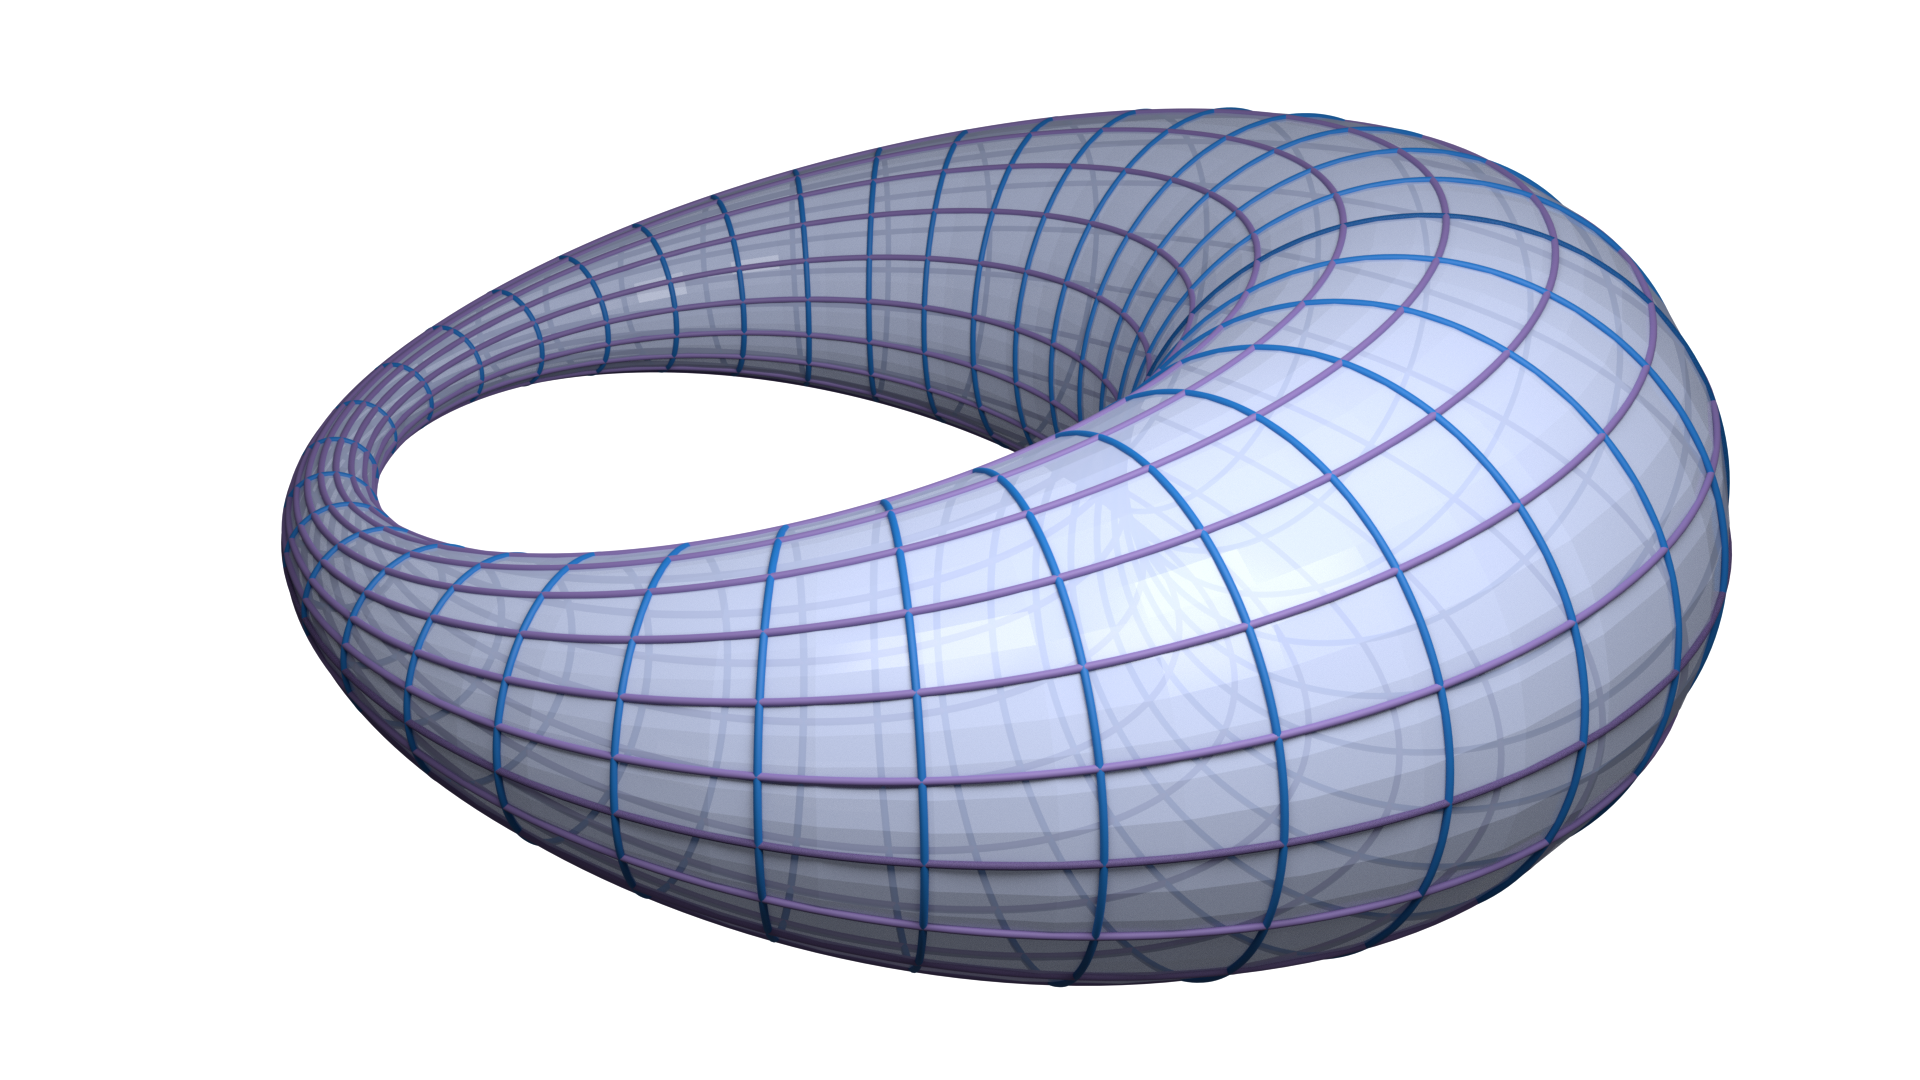
\includegraphics[width=\textwidth]{Dupin-net.png}
    \caption{Elliptical Dupin cyclide.}
    \label{fig:ellipto-hyperbolic-cyclides}
  \end{subfigure}
  \hfill
  \begin{subfigure}[b]{0.5\textwidth}
    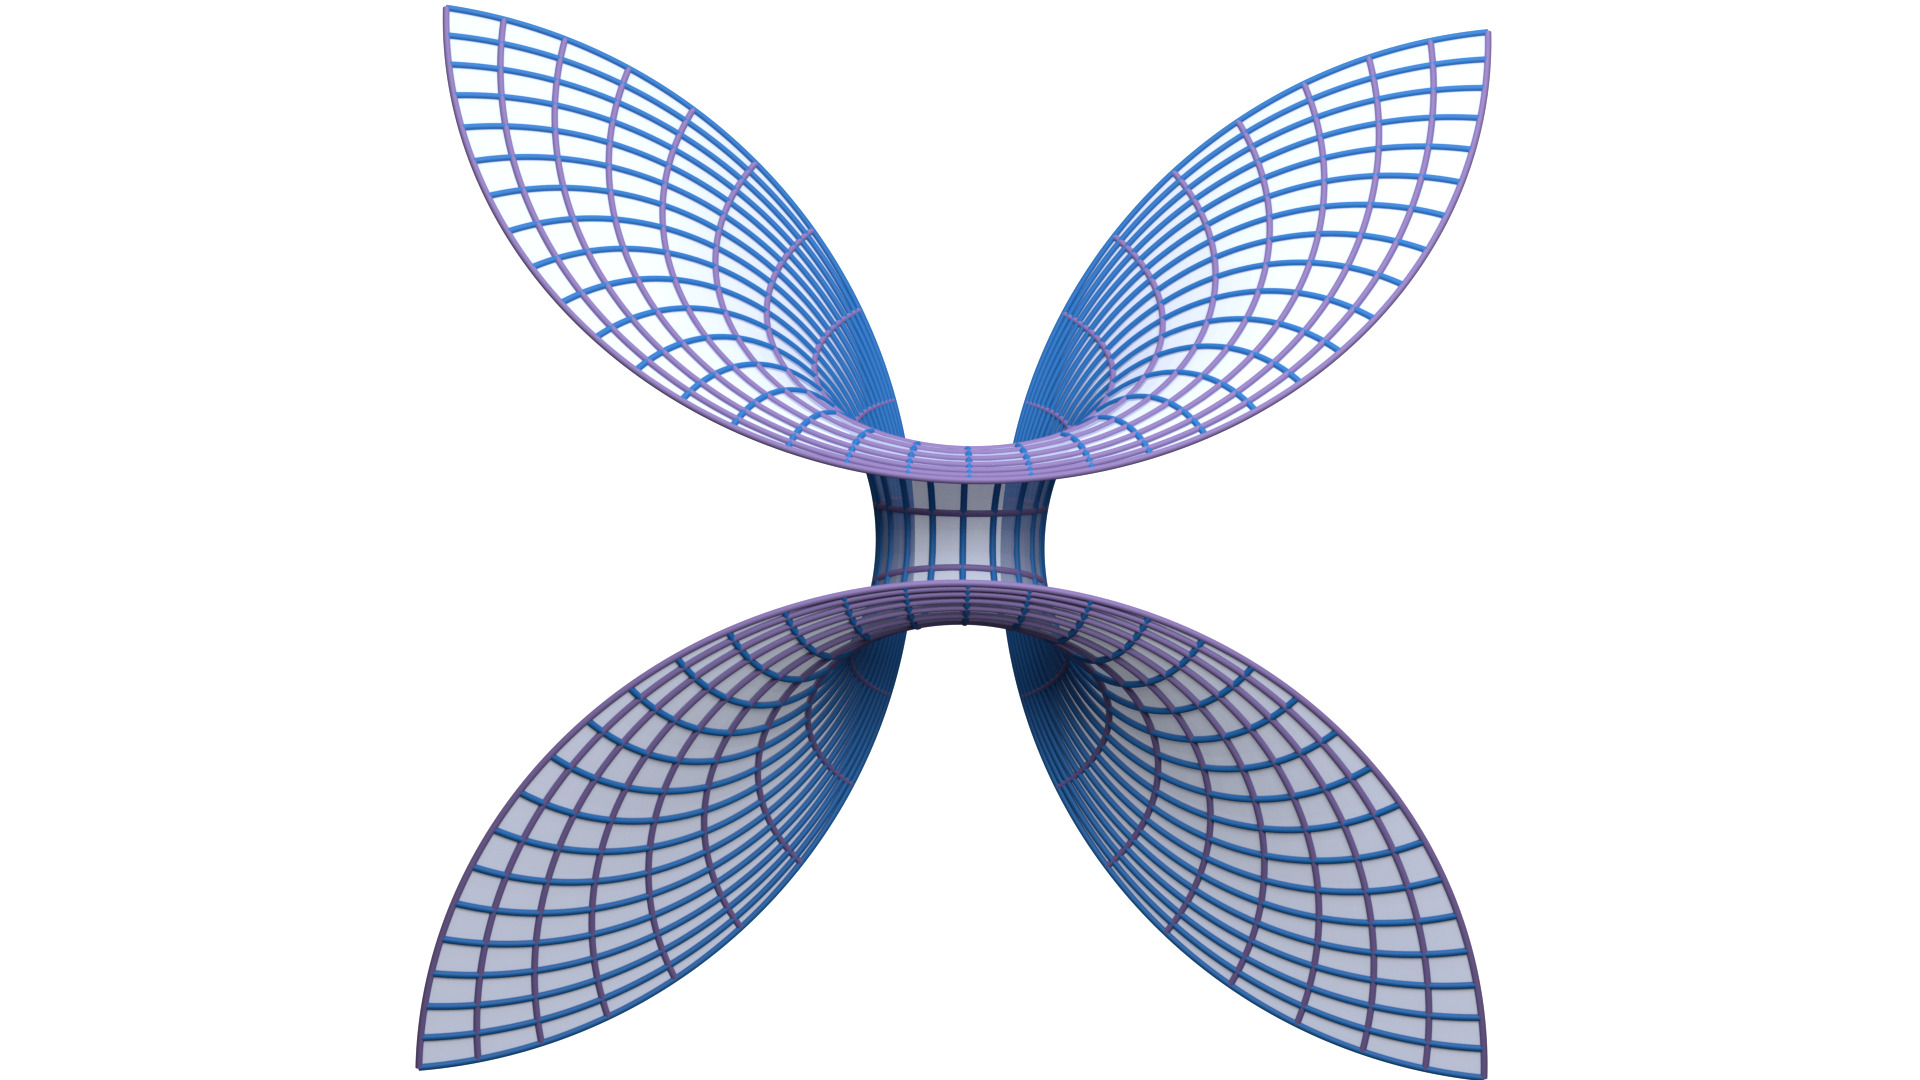
\includegraphics[width=\textwidth]{Dupin-net-2.png}
    \caption{Parabolic Dupin cyclide.}
    \label{fig:parabolic-cyclides}
  \end{subfigure}
  \caption{Nets on Dupin Cyclides.}
\end{figure}

\begin{example}
\label{ex:circular-sections-form-nets-on-quadrics}
In Section \ref{subsec:circles-on-quadrics} we proved that non-degenerate quadrics \textemdash with the exclusion of hyperbolic paraboloids, contain two circles through each point, and each circle lies in a one-parameter family of circular sections on the quadric. Thus, the circular sections form a net on quadrics.
\end{example}

\begin{definition}[Diagonally related nets on surfaces]
\label{def:diag-nets-on-surfaces}
Let $\mathcal{N}_{1}$ and $\mathcal{N}_{2}$ be two nets on a surface $\Sigma$. Then $\mathcal{N}_{2}$ is called diagonal
to $\mathcal{N}_{1}$ if the following condition is satisfied whenever any four curves of $\mathcal{N}_{1}$ form a
(combinatorial) quadrilateral: \newline
If one pair of opposite vertices is connected by a curve from $\mathcal{N}_{2}$, then the other pair of opposite vertices is connected by a curve from $\mathcal{N}_{1}$.
\end{definition}

\begin{figure}[H]
    \centering
    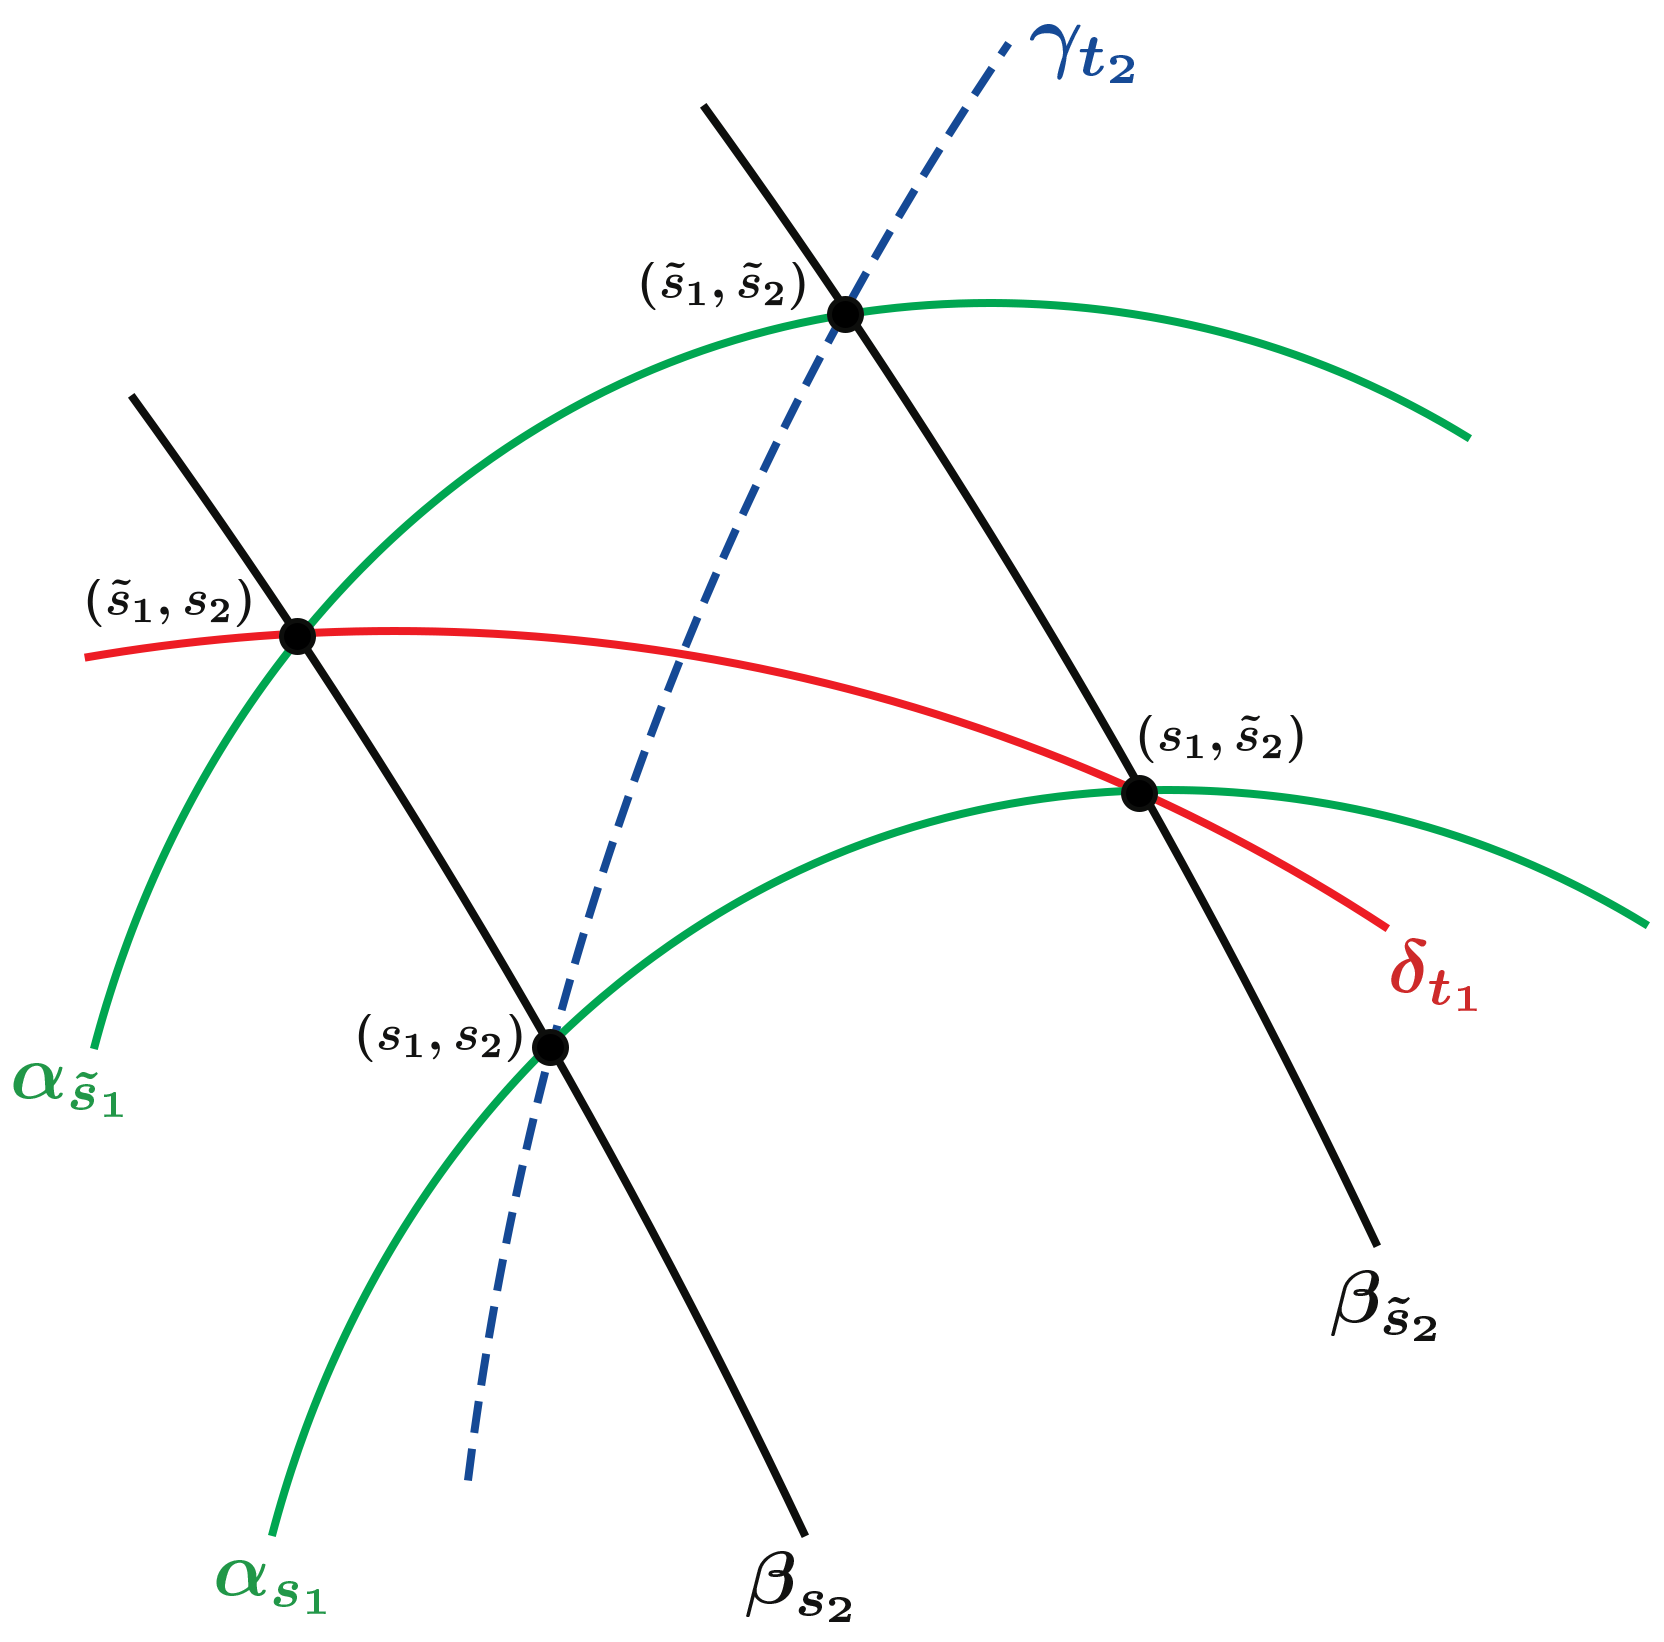
\includegraphics[width=0.5\textwidth]{diagonally_related_diagram.png}
    \caption{An illustration of the diagonal relation between two nets.}
    \label{fig:diagonally-related-diagram}
\end{figure}

\begin{theorem}
\label{thm:symmetric-definition-diagonal-nets}
Let $\mathcal{N}_1$ and $\mathcal{N}_2$ be two nets on a surface $\Sigma$. Then $\mathcal{N}_1$ is diagonally related to
$\mathcal{N}_2$ if and only if $\mathcal{N}_2$ is diagonally related to $\mathcal{N}_1$.
\end{theorem}

\begin{proof}
    See \cite[\textcolor{CitationColor}{Theorem~8.2.}]{geometryIII}.
\end{proof}

\begin{remark}
\label{rm:plusminus}
Let $\varphi : I_{2} \times I_{2} \to \mathbb{R}^3$ be a parameterization of a surface. We have seen in Example~\ref{ex:coordinate-lines-form-net-on-surfaces}, that its coordinate lines define a net $\mathcal{N}_{\varphi}$ on $\varphi(I_{1} \times I_{2})$ in $\mathbb{R}^3$. Define
\[
    s_{1} := u + v \quad \text{and} \quad s_{2} := u - v.
\]
Then these new variables generate the parameterization:
\[
    \boldsymbol{x}(s_{1}, s_{2}) = \varphi\left(u + v, u - v \right).
\]
Consider any quadrilateral formed by the curves of $\mathcal{N}_{\varphi}$. If the points $(u_{1}, v_{1})$ and $(u_{2}, v_{2})$ have the same $s_{1}$ coordinate, i.e. one pair of opposite vertices is connected by a curve from $\mathcal{N}_{\boldsymbol{x}}$. Then
\[
    s_{1} = u_{1} + v_{1} = u_{2} + v_{2},
\]
or equivalently, $u_{1} - v_{2} = u_{2} - v_{1}$. This implies that $(u_{2}, v_{1})$ and $(u_{1}, v_{2})$ have the same $s_{2}$ coordinate. Thus, the nets corresponding to each parameterization are diagonally related.
\end{remark}

\subsection{Diagonally related nets on hyperboloids}
We are now ready to determine the relationship between the lines of curvature and circular sections on one- and two- sheeted hyperboloids.

\begin{theorem}[]
\label{thm:diagonally-related-one-sheeted}
On any one-sheeted hyperboloid, the net of curvature lines and the net of circular sections are diagonally related.
\end{theorem}
\begin{proof}
Let $\mathcal{H}$ denote the one-sheeted hyperboloid
\[
    \mathcal{H} \; : \; \frac{x^2}{\alpha} + \frac{y^2}{\beta} - \frac{z^2}{\gamma} = 1.
\]
with $\alpha, \beta, \gamma > 0$, and $\alpha > \beta$. Set $a := \alpha$, $b := \beta$, and $c := -\gamma$. Then the triple $a, b, c$ with $a > b > c$ determine the confocal family of quadrics
\[
    \mathcal{Q}_{\lambda} \; : \; \frac{x^2}{a+\lambda} + \frac{y^2}{b+\lambda} + \frac{z^2}{c+\lambda} = 1,
\]
and $\mathcal{H}$ can be recovered from $\mathcal{Q}_{\lambda}$ for $\lambda = 0$. Consequently, the confocal coordinate system defined by (\ref{eq:main-parameterization}) yields a curvature line parameterization of $\mathcal{H}$ for
\[
    u_{2}(s_{2}) = 0,
\]
or equivalently,
\[
    f_{2}(s_{2})^2 = a = \alpha, \quad g_{2}(s_{2})^2 = b = \beta, \quad h_{2}(s_{2})^2 = -c = \gamma.
\]
Thus, the parametrization can be written as
\begin{equation}
\begin{aligned}
\label{eq:diagonal-h1-parameterization}
    x &= \frac{\sqrt{\alpha} \ f_{1} f_{3}}{\sqrt{\alpha - \beta}\sqrt{\alpha + \gamma}}, \\
    y &= \frac{\sqrt{\beta} \ g_{1} g_{3}}{\sqrt{\alpha - \beta}\sqrt{\beta + \gamma}}, \\
    z &= \frac{\sqrt{ \gamma } \ h_{1} h_{3}}{\sqrt{\alpha + \gamma}\sqrt{\beta + \gamma}},
\end{aligned}
\end{equation}
with
\begin{equation}
\begin{aligned}
\label{eq:functional-relations-h1}
    f_{1}(s_{1})^2 + g_{1}(s_{1})^2 &= \alpha - \beta, \quad f_{1}(s_{1})^2 + h_{1}(s_{1})^2 = \alpha + \gamma \\
    f_{3}(s_{3})^2 - g_{3}(s_{3})^2 &= \alpha - \beta, \quad f_{3}(s_{3})^2 - h_{3}(s_{3})^2 = \alpha + \gamma.
\end{aligned}
\end{equation}
We show that there exists functions $f_1, g_1, h_1, f_3, g_3, h_3$, such that the diagonal net given by the coordinate lines of (\ref{eq:diagonal-h1-parameterization})
\[
    s_{\pm} := s_{1} \pm s_{3}
\]
are the circular cross sections of the the hyperboloid. Substituting the parametrization (\ref{eq:diagonal-h1-parameterization}) into the equations of the planes (\ref{eq:planes-one-sheeted}) yields the functional equation
\begin{equation}
\label{extra-plane-equation-h1}
    g_1(s_{1}) g_3(s_{3}) \pm h_1(s_{1}) h_3(s_{3}) = \frac{\sqrt{\beta+\gamma}}{\sqrt{\gamma \beta }} \lambda_{\pm}
\end{equation}
For the diagonal lines $s_{\pm} = \text{const.}$ to lie these planes, the parameters $\lambda_{+}$ and $\lambda_{-}$ must be functions of $s_{+}$ and $s_{-}$ only, respectively. Thus, $f_1, g_1, f_3, g_3$ must satisfy the functional system:
\begin{equation*}
\begin{aligned}
h_1(s_{1})^2 - g_1(s_{1})^2 &= \beta  + \gamma \\
g_3(s_{3})^2 - h_3(s_{3})^2 &= \beta  + \gamma \\
g_1(s_{1}) g_3(s_{3}) \pm h_1(s_{1}) h_3(s_{3}) &= \frac{\sqrt{\beta+\gamma}}{\sqrt{\gamma \beta }} \lambda_{\pm}(s_1 \pm s_3),
\end{aligned}
\end{equation*}
which is readily solved by hyperbolic functions:
\begin{equation*}
\begin{aligned}
g_{1}(s_{1}) &= \sqrt{\beta+\gamma} \sinh(s_{1}) \quad g_{3}(s_{3}) = \sqrt{\beta+\gamma} \cosh(s_{3}) \\
h_{1}(s_{1}) &= \sqrt{\beta+\gamma} \cosh(s_{1}) \quad h_{3}(s_{3}) = \sqrt{\beta+\gamma} \sinh(s_{3}).
\end{aligned}
\end{equation*}
The last two equations follow from the addition and subtraction laws
\begin{align*}
\sinh(x \pm y) = \sinh(x) \cosh(y) \pm \cosh(x) \sinh(y),
\end{align*}
and therefore, $\lambda_{\pm}$ are given by
\[
\lambda_{\pm} = \sqrt{ \gamma \beta (\beta \pm \gamma) } \sinh(s_{1} \pm s_{3}).
\]
Now we obtain $f_{1}$ and $f_{3}$ from the fundamental relations (\ref{eq:functional-relations-h1}).
\begin{align}
f_{1}(s_{1})^2 &= \alpha-\beta-(\beta+\gamma)\sinh^2(s_{1}), \label{eq:solution-of-f1} \\
f_{3}(s_{3})^2 &= \alpha+\gamma+(\beta+\gamma)\sinh^2(s_{3}). \label{eq:solution-of-f3}
\end{align}
The right hand side of Equation (\ref{eq:solution-of-f1}) is non-negative for $s_{1} \in [-s_{1}^{0}, s_{1}^{0}]$ with
\[
    s_{1}^{0} = \sinh^{-1}\left( \sqrt{\frac{\alpha - \beta}{\gamma - \beta}} \right),
\]
Since the inverse hyperbolic $\sinh$ is defined for all of $\mathbb{R}$, the value $s_{1}^{0}$ is well-defined. Note also that there are no restriction on the domain of the $s_{3}$ parameter. Thus, it can be varied freely on any arbitrary interval $I \subseteq \mathbb{R}$. \par
Since $f_{1}$ and $f_{3}$ are determined by the square roots of (\ref{eq:solution-of-f1}-\ref{eq:solution-of-f3}), we obtain two separate parameterizations for the hyperboloid $\mathcal{H}$, one for $x > 0$, and another for $x < 0$:
\[
    \varphi_{\pm} \; : \; [-s_{1}^{0}, s_{1}^{0}] \times I \to \mathbb{R}^3, \quad \quad (s_{1}, s_{3}) \mapsto \begin{pmatrix}
        x(s_{1}, s_{3}) \\
        y(s_{1}, s_{3}) \\
        z(s_{1}, s_{3})
        \end{pmatrix}
\]
with
\begin{align*}
x(s_{1}, s_{3}) &= \pm \sqrt{\alpha} \sqrt{1-\frac{\beta + \gamma}{\alpha - \beta}\sinh^2(s_{1})} \sqrt{1 + \frac{\beta+\gamma}{\alpha+\gamma }\sinh^2(s_{3})}, \\
y(s_{1}, s_{3}) &= \sqrt{\frac{\beta (\beta + \gamma)}{\alpha - \beta}} \sinh(s_{1}) \cosh(s_{3}), \\
z(s_{1}, s_{3}) &= \sqrt{\frac{\gamma (\beta + \gamma)}{\alpha + \gamma}} \cosh(s_{1}) \sinh(s_{3}).
\end{align*}
Note that each parameterization covers its half of the hyperboloid entirely, i.e. the boundary at $x = 0$ is reached, and thus considered together, they cover the entire hyperboloid. By construction, the net of curvature lines of an arbitrary one-sheeted hyperboloid is digonally-related to its net of circular sections.
\end{proof}

\begin{theorem}[]
\label{thm:diagonally-related-two-sheeted}
On any two-sheeted hyperboloid, the net of curvature lines and the net of circular sections are diagonally related.
\end{theorem}
\begin{proof}
Let $\mathcal{H}$ denote the two-sheeted hyperboloid
\[
    \mathcal{H} \; : \; \frac{x^2}{\alpha} - \frac{y^2}{\beta} - \frac{z^2}{\gamma} = 1.
\]
with $\alpha, \beta, \gamma > 0$, and $\gamma > \beta$. Set $a := \alpha$, $b := -\beta$, and $c := -\gamma$. Then the triple $a, b$, and $c$ satisfy $a > b > c$. Thus, they determine the confocal family of quadrics
\[
    \mathcal{Q}_{\lambda} \; : \; \frac{x^2}{a+\lambda} + \frac{y^2}{b+\lambda} + \frac{z^2}{c+\lambda} = 1,
\]
The two-sheeted hyperboloid $\mathcal{H}$ can be recovered from $\mathcal{Q}_{\lambda}$ for $\lambda = 0$. Consequently, the confocal coordinate system defined by (\ref{eq:main-parameterization}) yields a curvature line parameterization of $\mathcal{H}$ for
\[
    u_{1}(s_{1}) = 0,
\]
or equivalently,
\[
    f_{1}(s_{1})^2 = a = \alpha, \quad -g_{1}(s_{1})^2 = b = -\beta, \quad -h_{1}(s_{1})^2 = c = -\gamma.
\]
Thus, the parametrization can be written as
\begin{equation}
\begin{aligned}
\label{eq:diagonal-h2-parameterization}
    x &= \frac{\sqrt{\alpha} \ f_{2} f_{3}}{\sqrt{\alpha + \beta}\sqrt{\alpha + \gamma}}, \\
    y &= \frac{\sqrt{\beta} \ g_{2} g_{3}}{\sqrt{\alpha + \beta}\sqrt{\gamma - \beta}}, \\
    z &= \frac{\sqrt{ \gamma } \ h_{2} h_{3}}{\sqrt{\alpha + \gamma}\sqrt{\gamma - \beta}},
\end{aligned}
\end{equation}
with
\begin{equation}
\begin{aligned}
\label{eq:functional-relations-h2}
f_{2}(s_{2})^2 - g_{2}(s_{2})^2 &= a - b, \quad f_{2}(s_{2})^2 + h_{2}(s_{2})^2 = a - c \\
f_{3}(s_{3})^2 - g_{3}(s_{3})^2 &= a - b, \quad f_{3}(s_{3})^2 - h_{3}(s_{3})^2 = a - c
\end{aligned}
\end{equation}
Following the same approach as in the proof of Theorem~\ref{thm:diagonally-related-one-sheeted}, we want to show that there exists functions $f_2, g_2, h_2, f_3, g_3, h_3$, such that the diagonal net given by the coordinate lines of (\ref{eq:diagonal-h2-parameterization})
\[
    s_{\pm} := s_{2} \pm s_{3}
\]
are the circular cross sections of the the hyperboloid. Substituting the parametrization (\ref{eq:diagonal-h2-parameterization}) into the equations of the planes (\ref{eq:planes-two-sheeted}) yields the functional equations
\begin{equation}
\label{extra-plane-equation-h2}
f_{2}(s_{2}) f_{3}(s_{3}) \pm g_{2}(s_{2}) g_{3}(s_{3}) = \frac{\sqrt{\alpha+\beta}}{\sqrt{\alpha} \sqrt{\beta}} \lambda_{\pm}(s_{2} \pm s_{3})
\end{equation}
Again, for the diagonal lines $s_{\pm} = \text{const.}$ to lie these planes, the parameters $\lambda_{+}$ and $\lambda_{-}$ must depend only on $s_{+}$ and $s_{-}$, respectively. Thus, $f_2, g_2, f_3, g_3$ must satisfy the functional system:
\begin{equation*}
\begin{aligned}
f_{2}^2(s_{2}) - g_{2}^2(s_{2}) &= \alpha + \beta, \\
f_{3}^2(s_{3}) - g_{3}^2(s_{3}) &= \alpha + \beta, \\
f_{2}(s_{2}) f_{3}(s_{3}) \pm g_{2}(s_{2}) g_{3}(s_{3}) &= \frac{\sqrt{\alpha+\beta}}{\sqrt{\alpha} \sqrt{\beta}} \lambda_{\pm}(s_{2} \pm s_{3}),
\end{aligned}
\end{equation*}
which is once again solved by hyperbolic functions:
\begin{equation*}
\begin{aligned}
f_{2}(s_{2}) &= \sqrt{\alpha + \beta} \cosh(s_{2}) & g_{2}(s_{2}) &= \sqrt{\alpha + \beta} \sinh(s_{2}) \\
f_{3}(s_{3}) &= \sqrt{\alpha + \beta} \cosh(s_{3}) & g_{3}(s_{3}) &= \sqrt{\alpha + \beta} \sinh(s_{3})
\end{aligned}
\end{equation*}
with
\[
\lambda_{\pm}(s_{2} \pm s_{3}) = \sqrt{ \alpha \beta (\alpha + \beta) } \cosh(s_{2} \pm s_{3})
\]
Now we obtain $h_{2}$ and $h_{3}$ from the fundamental relations (\ref{eq:functional-relations-h2}).
\begin{align}
h_{2}(s_{2})^2 &= \gamma - \beta - (\alpha + \beta) \sinh^2(s_{2}) \label{eq:solution-of-h2} \\
h_{3}(s_{3})^2 &= (\alpha + \beta) \sinh^2(s_{3}) + \beta - \gamma \label{eq:solution-of-h3}
\end{align}
The right hand side of Equation (\ref{eq:solution-of-h2}) is non-negative for $s_{2} \in [-s^{0}, s^{0}]$ with
\[
    s^{0} = \sinh^{-1}\left( \sqrt{\frac{\gamma - \beta}{\alpha + \beta}} \right),
\]
while the right hand side of Equation (\ref{eq:solution-of-h3}) is non-negative for $s_{3} \in [s_{0}, \infty)$. Perhaps a useful intuition for the domain of parameter $s_{3}$ is that, one can think of two sheets of hyperboloid \textemdash considered together, as a single ellipsoid joined at infinity. \par
Since $h_{2}$ and $h_{3}$ are determined by the square roots of (\ref{eq:solution-of-h2}-\ref{eq:solution-of-h3}), we obtain two separate parameterizations for each sheet of the hyperboloid $\mathcal{H}$, one for $z > 0$, and another for $z < 0$. The parametrizations of the sheet $\mathcal{H} \cap \{ (x, y, z) \in \mathbb{R}^3 : x > 0\}$ is given by
\[
    \varphi^{+}_{\pm} \; : \; [-s^{0}, s^{0}] \times [-s^{0}, \infty) \to \mathbb{R}^3, \quad \quad (s_{2}, s_{3}) \mapsto \begin{pmatrix}
        x(s_{2}, s_{3}) \\
        y(s_{2}, s_{3}) \\
        z(s_{2}, s_{3})
        \end{pmatrix}
\]
with
\begin{align*}
    x(s_2, s_3) &= \frac{\sqrt{\alpha (\alpha + \beta)}}{\sqrt{\alpha + \gamma}} \cosh(s_2) \cosh(s_3), \\
    y(s_2, s_3) &= \frac{\sqrt{\beta (\alpha + \beta)}}{\sqrt{\gamma + \beta}} \sinh(s_2) \sinh(s_3), \\
    z(s_2, s_3) &= \pm \frac{\sqrt{\gamma} \sqrt{\beta - \gamma}}{\sqrt{\alpha + \gamma}} \sqrt{1 - \frac{\alpha + \beta}{\gamma - \beta} \sinh^2(s_{2})} \sqrt{\frac{\alpha + \beta}{\beta - \gamma} \sinh^2(s_{3}) + 1}.
\end{align*}
Similarly, for the other sheet: $\varphi^{-}_{\pm}(s_2, s_3) = \left(-x(s_{2}, s_{3}), y(s_{2}, s_{3}), \pm z(s_{2}, s_{3}) \right)$.
For the values of parameters $s_{2}$ and $s_{3}$ given, each parameterization covers its half (of the sheet) of the hyperboloid entirely, including the boundary at $z = 0$. Therefore, the entire two-sheeted hyperboloid is covered.
\end{proof}
\pagebreak
%===========================================================
\section{Isometric deformation of circular cross sections of hyperboloids}
\label{sec:isometric-deformation}
\begin{proposition}
\label{prop:affine-transformation-one-sheeted}
Let $\alpha, \beta, \gamma > 0$ with $\alpha > \beta$, and define the one-sheeted hyperboloid:
\[
    \mathcal{H}: \frac{x^2}{\alpha} + \frac{y^2}{\beta} - \frac{z^2}{\gamma} = 1.
\]
Then, there exists a one-parameter family of affine transformations of $\mathbb{R}^3$ given by
\[
    (x, y, z) \mapsto (x, \sigma_{2}y, \sigma_{3}z)
\]
with $\sigma_{2}, \sigma_{3} > 0$, and
\begin{equation}
\label{eq:sigmas-h1}
    \beta(\alpha + \gamma) \sigma_{2}^2 + \gamma(\alpha - \beta) \sigma_{3}^2 = \alpha (\beta + \gamma)
\end{equation}
that is isometric on the circular sections of $\mathcal{H}$. Futhermore, all affine transforms of $\mathcal{H}$ under this map are confocal up to scaling.
\end{proposition}

\begin{proof}
Let $\sigma_{1}, \sigma_{2}, \sigma_{3} > 0$. We explicity construct a one-parameter affine transformations that is isometric on the circular sections of $\mathcal{H}$. Consider the candidate family:
\begin{equation*}
\label{eq:affine-transformation-h1}
    (x, y, z) \mapsto (\sigma_{1}x, \sigma_{2}y, \sigma_{3}z),
\end{equation*}
and let $S$ denote its matrix in homogeneous coordinates:
\[
    S = \begin{bmatrix}
        \sigma_{1} && 0 && 0 && 0 \\
        0 && \sigma_{2} && 0 && 0 \\
        0 && 0 && \sigma_{3} && 0 \\
        0 && 0 && 0 && 1
    \end{bmatrix}.
\]
Identify $\mathcal{H}$ with its Gram matrix
\[
    \mathcal{H} = \begin{bmatrix}
        1 / \alpha && 0 && 0 && 0 \\
        0 && 1 / \beta && 0 && 0 \\
        0 && 0 && -1 / \gamma && 0 \\
        0 && 0 && 0 && 1
    \end{bmatrix}.
\]
Then $\mathcal{H}$ transforms under $S$ by $\tilde{\mathcal{H}} = S^{\top}\mathcal{H}S$, i.e.
\[
\tilde{\mathcal{H}} \; : \; \frac{x^2}{\sigma_{1}^2\alpha} + \frac{y^2}{\sigma_{2}^2\beta} - \frac{z^2}{\sigma_{3}^2\gamma} = 1.
\]
Let $\Pi_{\pm}(\lambda_{\pm})$ denote the planes of the circular sections of $\mathcal{H}$ given by Equation (\ref{eq:planes-one-sheeted}) with normal vectors
\[
    n_{\pm} = \left[0, \sqrt{ \gamma (\alpha- \beta) }, \pm \sqrt{\beta(\alpha+\gamma)}, 1 \right].
\]
One immediately sees that $\Pi_{\pm}(\lambda_{\pm})$ are orthogonal to the coordinate plane $\{ x = 0 \}$ in $\mathbb{R}^3$. Since the normals transform under $S$ by $S^{-\top} n_{\pm}$, it follows that the planes remain orthogonal to the $\{ x = 0 \}$ coordinate plane after the transformation. \par
Due to the parallelity of the planes $\Pi_{\pm}(\lambda_{\pm})$, it's enough to consider a single plane in only one of the families, e.g. $\Pi_{+}(\lambda_{+})$ passing through the origin with $\lambda_{+} = 0$, and ensure that the candidate affine transformation is isometric on it. Let $\mathcal{C}$ denote the corresponding circle on $\Pi_{+}(0)$. Since it is (one of) the intersection circles of $\mathcal{H}$ with a two-fold contacting sphere centered at the origin [Figure~\ref{fig:proof-one-sheeted-transformation}], it follows that its center is the origin, and its radius is $\sqrt{\alpha}$. Thus, any candidate affine transformation that is isometric along the circular sections of $\mathcal{H}$ must preserve that radius. This directly implies that $\sigma_{1} = 1$. \par
Pick a point lying on $\mathcal{C}$ and on the orthogonal coordinate plane $\{x = 0\}$. Then its coordinates $(0, y, z)$ satisfy:
\[
    y^2 + z^2 = \alpha, \quad \text{and} \quad \frac{y^2}{\beta} - \frac{z^2}{\gamma} = 1.
\]
Solving for $y^2$ and $z^2$ yields
\[
    y^2 = \frac{\beta(\alpha + \gamma)}{\beta + \gamma}, \quad z^2 = \frac{\gamma(\alpha - \beta)}{\beta + \gamma}.
\]
Any affine transformation is an isometry on $\Pi_{+}(0)$ if and only if
\[
    z^2 + y^2 = \alpha = \tilde{y}^2 + \tilde{z}^2 = \sigma_{2}^2 y^2 + \sigma_{3}^2 z^2 = \sigma_{2}^2 \frac{\beta(\alpha + \gamma)}{\beta + \gamma} + \sigma_{3}^2 \frac{\gamma(\alpha - \beta)}{\beta + \gamma},
\]
which is equivalent to the equation
\begin{equation*}
    \alpha (\beta + \gamma) = \sigma_{2}^2 \beta(\alpha + \gamma) + \sigma_{3}^2 \gamma(\alpha - \beta).
\end{equation*}
If we set $\sigma_{2} = r$ such that $r \in [-r_0, r_0]$ with
\[
    r_{0} = \sqrt{\frac{\alpha (\beta + \gamma)}{\beta (\alpha + \gamma)}},
\]
Then $\sigma_3$ is given by
\[
    \sigma_{3} = \pm \sqrt{\frac{\alpha(\beta + \gamma) - \beta(\alpha + \gamma)r^2}{\gamma(\alpha - \beta)}}.
\]
Thus, we have constructed a one-parameter family of affine transformations with parameter $r$, that is isometric on the circular sections of $\mathcal{H}$. \par
Now, let $\tilde{\mathcal{H}}$ be an affine transform of $\mathcal{H}$ under the map given above. Then $\mathcal{H}$ and $\tilde{\mathcal{H}}$ are confocal up to scaling if and only if there exists $\mu > 0$ such that
\[
    \alpha - \sigma^2_{2} \beta = \mu (\alpha - \beta), \quad \text{and} \quad \alpha - \sigma_{3}^2 \gamma = \mu (\alpha - \gamma).
\]
From Equation (\ref{eq:sigmas-h1}), we get
\begin{align*}
\alpha - \sigma^2_{2} \beta &=  \alpha - \left( \frac{\alpha (\beta + \gamma)}{\alpha + \gamma} -  \frac{\gamma \sigma^2_{3} (\alpha - \beta)}{\alpha + \gamma} \right) \\
&= \frac{\alpha (\alpha + \gamma)}{\alpha + \gamma} + \frac{\gamma \sigma^2_{3} (\alpha - \beta)}{\alpha + \gamma} - \frac{\alpha (\beta + \gamma)}{\alpha + \gamma} \\
&= \frac{\alpha (\alpha - \beta) + \gamma \sigma^2_{3} (\alpha - \beta)}{\alpha + \gamma} \\
&= \frac{\alpha + \gamma \sigma^2_{3}}{\alpha + \gamma} (\alpha - \beta) \numberthis \label{eq:confocals-h1-last}
\end{align*}
Similarly,
\[
\alpha - \sigma_{3}^2 \gamma = \frac{\alpha - \sigma^2_{2} \beta}{\alpha - \beta}(\alpha - \gamma) = \frac{\alpha + \gamma \sigma^2_{3}}{\alpha + \gamma} (\alpha - \gamma)
\]
where the last equality follows from (\ref{eq:confocals-h1-last}).
\end{proof}

\begin{figure}[H]
    \centering
    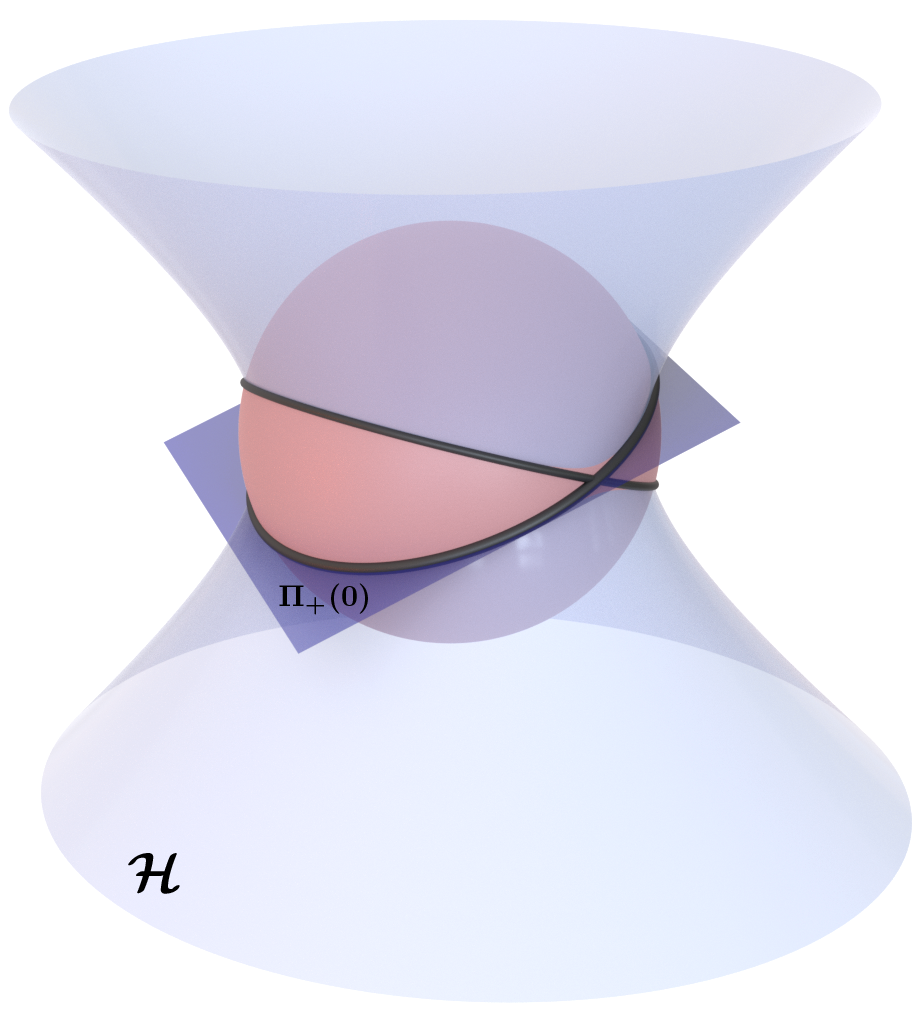
\includegraphics[width=0.5\textwidth]{proof-one-sheeted-transformation.png}
\caption[One-sheeted hyperboloid and a sphere centered at the origin intersect in two circles.]{A one-sheeted hyperboloid with first principal axis $\alpha$ and a sphere centered at the origin intersect in two circles $\mathcal{C}_1$, and $\mathcal{C}_2$ with radii equal to $\sqrt{\alpha}$}
    \label{fig:proof-one-sheeted-transformation}
\end{figure}

As an extension of Proposition~\ref{prop:affine-transformation-one-sheeted}, we now construct a one-parameter family of curvature line parametrizations of a one-sheeted hyperboloid, which describes the isometric deformation of the circular cross-sections.

\begin{theorem}
\label{thm:isometric-deformation-para-one-hyperboloid}
Let $a > b > c > 0$ and $\mathcal{H}(s_{2})$ be a one-parameter family of one-sheeted hyperboloids given by
\begin{equation*}
x^2 + \frac{a - c}{b - c} \frac{y^2}{\sin(s_{2})^2} -  \frac{a - b}{b - c} \frac{z^2}{ \cos(s_{2})^2} = 1.
\end{equation*}
Then for each $s_{2} \in \left[ 0, \frac{\pi}{2} \right]$, the two parameterizations
\begin{align*}
    \varphi_{\pm} &: [-s_{1}^{0}, s_{1}^{0}] \times (-\infty, \infty) \to \mathbb{R}^3, \quad \quad (s_{1}, s_{3}) \mapsto (x, y, z) \\[10pt]
    x(s_{1}, s_{2}, s_{3}) &= \pm \sqrt{1 - \frac{b - c}{a - b} \sinh^2(s_{1})} \sqrt{1 + \frac{b - c}{a - c}\sinh^2(s_{3})} \\[10pt]
    y(s_{1}, s_{2}, s_{3}) &= \frac{b - c}{\sqrt{a - b} \sqrt{a - c}} \sinh(s_{1}) \sin(s_{2})\cosh(s_{3}) \\[10pt]
    z(s_{1}, s_{2}, s_{3}) &= \frac{b - c}{\sqrt{a - b} \sqrt{a - c}}  \cosh(s_{1}) \cos(s_{2}) \sinh(s_{3})
\end{align*}
with
\[
    s_{1}^{0} = \sinh^{-1}\left( \sqrt{ \frac{a - b}{b - c} } \right)
\]
\sloppy are curvature line parameterizations of the two halves ${\mathcal{H}(s_{2}) \cap \{ x \geq 0\}}$ and ${\mathcal{H}(s_{2}) \cap \{ x \leq 0\}}$ of the one-sheeted hyperboloid, and the curves $s_{1} \pm s_{3} = \text{const.}$ are congruent circles. \newline
This one-parameter family of one-sheeted hyperboloids $\mathcal{H}_{1}(s_{2})$ includes two planar degenerations corresponding to $s_{2} = 0,\left(y = 0 \right)$ and $s_{2} = \pi/2, \left( z = 0 \right)$.
\end{theorem}

\begin{proof}
    Let $\alpha, \beta, \gamma > 0$ with $\alpha > \beta$. Let $\mathcal{H}$ denote a one-sheeted hyperboloid transformed under ${(x, y, z) \mapsto (x, \sigma_2 y, \sigma_3 z)}$ as given in Proposition~\ref{prop:affine-transformation-one-sheeted}, and further scale it to have its first semi-axis equal to $1$:
\[
\mathcal{H} \; : \; x^2 + \frac{\alpha y^2}{\sigma_{2}^2 \beta} - \frac{\alpha z^2}{\sigma_{3}^2 \gamma} = 1.
\]
Now consider the one-parameter families of one-sheeted hyperboloids, which are obtained by uniformly scaling the hyperboloids of a system of confocal quadrics:
\[
x^2 + \frac{(u_{2} + a)y^2}{(u_{2} + b)} + \frac{(u_{2} + a)z^2}{(u_{2} + c)} = 1,
\]
for $u_{2} \in (-b, -c)$. Set $a = \alpha, b = \sigma_{2}^2 \beta, c = -\sigma_{3}^2 \gamma$. Then $\mathcal{H}$ is embedded in that family for $u_{2} = 0$. \par
Using the fundamental relations (\ref{eq:compatibility-conditions}), we can write the confocal family as
\begin{equation}
\label{eq:last-thm-h1-confocal}
x^2 + \frac{f_{2}(s_{2})^2 y^2}{g_{2}(s_{2})^2} - \frac{f_{2}(s_{2})^2 z^2}{h_{2}(s_{2})^2} = 1
\end{equation}
Let $\hat{g}_{2}(s_{2}) = \frac{g_{2}(s_{2})}{f_{2}(s_{2})}$, and $\hat{h}_{2}(s_{2}) = \frac{h_{2}(s_{2})}{f_{2}(s_{2})}$. Then (\ref{eq:last-thm-h1-confocal}) can be rewritten in the form
\[
x^2 + \frac{y^2}{\hat{g}_{2}(s_{2})^2} -  \frac{z^2}{\hat{h}_{2}(s_{2})^2} = 1,
\]
where the functions $\hat{g}$ and $\hat{h}$ constitute the semi-axes of the hyperboloid, i.e.
\[
f_{2}(s_{2})^2 = \alpha, \quad \hat{g}_{2}(s_{2})^2 = \frac{\beta \sigma_{2}^2}{\alpha} \quad \hat{h}_{2}(s_{2})^2 = \frac{\gamma \sigma_{3} ^2}{\alpha}
\]
From Proposition~\ref{prop:affine-transformation-one-sheeted}, we know that they are related by Equation~(\ref{eq:sigmas-h1}), and thus $\hat{g}$ and $\hat{h}$ must satisfy
\[
\beta + \gamma = \hat{g}_{2}(s_{2})^2(\alpha + \gamma) + \hat{h}_{2}(s_{2})^2(\alpha - \beta),
\]
or equivalently in terms of the parameters of the confocal family $a, b$, and $c$:
\[
    b - c = \hat{g}_{2}(s_{2})^2(a - c) + \hat{h}_{2}(s_{2})^2(a - b)
\]
The curvature-line parameterization of the hyperboloid $\mathcal{H}$ in terms of the uniformly-scaled confocal family is given by
\begin{equation}
\begin{aligned}
\label{eq:confocal-h1-parameterization}
    x &= \frac{f_1 f_3}{\sqrt{a-b}\sqrt{a-c}}, \\
    y &= \frac{g_1 \hat{g}_{2} g_3}{\sqrt{a-b}\sqrt{b-c}}, \\
    z &= \frac{h_1 \hat{h}_{2} h_3}{\sqrt{a-c}\sqrt{b-c}},
\end{aligned}
\end{equation}
with
\begin{equation*}
\begin{aligned}
f_{1}(s_{1})^2 + g_{1}(s_{1})^2 &= a - b, \quad f_{1}(s_{1})^2 + h_{1}(s_{1})^2 = a - c, \quad h_{1}(s_{1})^2 - g_{1}(s_{1})^2 = b - c \\
f_{3}(s_{3})^2 - g_{3}(s_{3})^2 &= a - b, \quad f_{3}(s_{3})^2 - h_{3}(s_{3})^2 = a - c, \quad g_{3}(s_{3})^2 - h_{3}(s_{3})^2 = b - c
\end{aligned}
\end{equation*}
The equation relating $\hat{g}$ and $\hat{h}$ is readily solved by trigonometric functions:
\[
\hat{g}_{2}(s_{2}) = \frac{\sqrt{b - c}}{\sqrt{a - c}} \sin(s_{2}) \quad \quad \hat{h}_{2}(s_{2}) = \frac{\sqrt{b - c}}{\sqrt{a - b}} \cos(s_{2}).
\]
This implies that the parameter of the family of confocal one-sheeted hyperboloid $s_2$ is periodic. Now we solve for the rest of the functions:
\begin{equation*}
\begin{aligned}
g_{1}(s_{1}) &= \sqrt{b - c} \sinh(s_{1}), \quad h_{1}(s_{1}) = \sqrt{b - c} \cosh(s_{1}), \quad f_{1}(s_{1}) = \pm \sqrt{(a - b) - (b - c)\sinh^2(s_{1})} \\
g_{3}(s_{3}) &= \sqrt{b - c} \cosh(s_{3}), \quad h_{3}(s_{3}) = \sqrt{b - c} \sinh(s_{3}), \quad f_{3}(s_{3}) = \pm \sqrt{(a - c) + (b - c)\sinh^2(s_{3})}
\end{aligned}
\end{equation*}
\sloppy Substituting in Equations (\ref{eq:confocal-h1-parameterization}), we get the parameterizations of the two halves ${\mathcal{H} \cap \{ x \leq 0\}}$ and ${\mathcal{H} \cap \{ x \geq 0\}}$ in the form given in the statement of the Theorem. \par
As we have already shown in Proposition~\ref{prop:affine-transformation-one-sheeted}, the affine transformation defined by $\sigma_2$ and $\sigma_3$ preserves distances along the circular sections. It follows that for any one-sheeted hyperboloid in the family the curves $s_{1} \pm s_{3} = \text{const.}$ are congruent circles.
\end{proof}

\begin{figure}[H]
    \centering
    \includegraphics[width=1.0\textwidth]{h1-deformation.png}
    \caption[Isometric deformation of one-sheeted hyperboloid along circular sections.]{Diagonally related nets of curvature lines and circular sections on one-sheeted hyperboloid and its isometric deformation along circular sections.}
    \label{fig:h1-deform}
\end{figure}

\begin{proposition}
\label{prop:affine-transformation-two-hyperboloid}
Let $\alpha > \beta > \gamma > 0$ with $\gamma > \beta$, and define a two-sheeted hyperboloid by
\[
    \mathcal{H} \; : \; \frac{x^2}{\alpha} - \frac{y^2}{\beta} - \frac{z^2}{\gamma} = 1.
\]
Then, there exists a one-parameter family of affine transformations given by
\[
    (x, y, z) \mapsto (\sigma_{1}x, \sigma_{2}y, z)
\]
with $\sigma_{1}, \sigma_{2} > 0$, and
\begin{equation}
\label{eq:sigmas-h2}
    \beta (\alpha + \gamma) \sigma_{2}^2 - \alpha (\beta - \gamma) \sigma_{1}^2 = \gamma (\alpha + \beta)
\end{equation}
that is isometric on the circular sections of $\mathcal{H}$. Futhermore, all affine transforms of $\mathcal{H}$ under this map are confocal up to scaling.
\end{proposition}
\begin{proof}
Let $\sigma_{1}, \sigma_{2}, \sigma_{3} > 0$. Following the same approach as in the proof of Proposition~\ref{prop:affine-transformation-one-sheeted}, we consider a candidate family of one-parameter affine transformations
\begin{equation*}
\label{eq:affine-transformation-h2}
    (x, y, z) \mapsto (\sigma_{1}x, \sigma_{2}y, \sigma_{3}z),
\end{equation*}
that transforms $\mathcal{H}$ to the two-sheeted hyperboloid
\[
\tilde{\mathcal{H}} \; : \; \frac{x^2}{\sigma_{1}^2\alpha} - \frac{y^2}{\sigma_{2}^2\beta} - \frac{z^2}{\sigma_{3}^2\gamma} = 1.
\]
Let $\Pi_{\pm}(\lambda_{\pm})$ denote the planes of the circular sections of $\mathcal{H}$ (\ref{eq:planes-two-sheeted}). Their normal vectors are given by
\[
    n_{\pm} = \left[\sqrt{\beta} \ \sqrt{\alpha + \gamma}, \pm \sqrt{\alpha} \ \sqrt{\gamma - \beta}, 0, 1 \right].
\]
Thus, the planes transform under (\ref{eq:affine-transformation-h2}) into
\begin{equation}
\label{eq:transformed-plane-h2}
\tilde{\Pi}_{\pm}(\lambda_{\pm}) \; : \; \frac{\sqrt{\beta (\alpha + \gamma)}}{\sigma_{1}} x \pm \frac{\sqrt{\alpha (\gamma - \beta)}}{\sigma_{2}} y = \lambda_{\pm}
\end{equation}
For any fixed $\lambda_{0} = \lambda_{+} = \lambda_{-}$, the circular sections of the hyperboloid intersect in two points, $p_1$ and $p_2$ that lie mirror symmetric with respect to the the coordinate plane $\{z = 0\}$. Any affine transformations that is isometric on the circles must preserve the distance along the $z$-axis between these two intersection points. This implies that $\sigma_{3} = 1$. \par

Our goal now is to find the relation governing $\sigma_{1}$, and $\sigma_{2}$. We compute the affine coordinates of $p_{1}, p_2 \in \mathbb{R}^3$ in terms of $\alpha, \beta, \gamma, \lambda_{0}, \sigma_{1}$, and $\sigma_2$ to get
\[
p_{1} = \left( \frac{\sigma_{1} \lambda_{0}}{\sqrt{\beta (\alpha + \gamma)}}, 0, \sigma_{3} \sqrt{\gamma} \sqrt{ \frac{\lambda^2_{0}}{\alpha \beta (\alpha + \gamma)} - 1 } \right), \quad \text{and} \quad p_{2} = \left( \frac{\sigma_{1} \lambda_{0}}{\sqrt{\beta (\alpha + \gamma)}}, 0, -\sigma_{3} \sqrt{\gamma} \sqrt{ \frac{\lambda^2_{0}}{\alpha \beta (\alpha + \gamma)} - 1 } \right).
\]
Let $m$ denote midpoint of the line segment $p_{1} \vee p_{2}$. Then
\[
    m = \left( \frac{\sigma_{1} \lambda_{0}}{\sqrt{\beta (\alpha + \gamma)}}, 0, 0 \right).
\]
The circular section of each plane $\Pi_{\pm}\left(\lambda_{0}\right)$ intersects the symmetry coordinate plane $\{z = 0\}$ in two points, which we denote by $q^{\pm}_{1}$, and $q^{\pm}_{2}$ [Figure~\ref{fig:proof-h2}]. Their coordinates $(x, y, z)$ satisfy the equations
\[
    \frac{x^2}{\alpha} - \frac{y^2}{\beta} - 1 = 0,
\]
and (\ref{eq:transformed-plane-h2}). Using a computer algebra system, we can explicity compute their coordinates in terms of $\alpha, \beta, \gamma, \lambda_{0}, \sigma_{1}$, and $\sigma_2$. \par
For the candidate affine transformation to be isometric in the plane of some circular section, it must preserve the distance between any two points on that plane, e.g. $d = \norm{q^{+}_{1} - q^{+}_{2}}$. Choosing $m$ to be one of these points yields a simpler equation for the distance. Again, using a computer algebra system, we equate the equation of the distance before the transformation with $\sigma_{1} = 1, \sigma_{2} = 1$, and after the transformation with an arbitrary $\sigma_{1}, \sigma_{2}$ to get the relation:
\begin{equation}
    \beta (\alpha + \gamma) \sigma_{2}^2 - \alpha (\beta - \gamma) \sigma_{1}^2 = \gamma (\alpha + \beta).
\end{equation}
If we set $\sigma_{1} = r$ such that $r \in [-r_0, r_0]$ with
\[
    r_{0} = \frac{\sqrt{\gamma (\alpha + \beta)}}{\lvert \alpha (b - c) \rvert },
\]
Then $\sigma_2$ is given by
\[
    \sigma_{2} = \pm \frac{\alpha (\beta - \gamma) r^2 + \gamma (\alpha + \beta)}{\beta (\alpha + \gamma)}.
\]
Thus, we have constructed a one-parameter family of affine transformations with parameter $r$, that is isometric on the circular sections of $\mathcal{H}$. In the exact manner shown in the proof of Proposition~\ref{prop:affine-transformation-one-sheeted}, one can again establish that all affine transforms of $\mathcal{H}$ under this map are confocal.
\end{proof}

\begin{figure}[H]
    \centering
    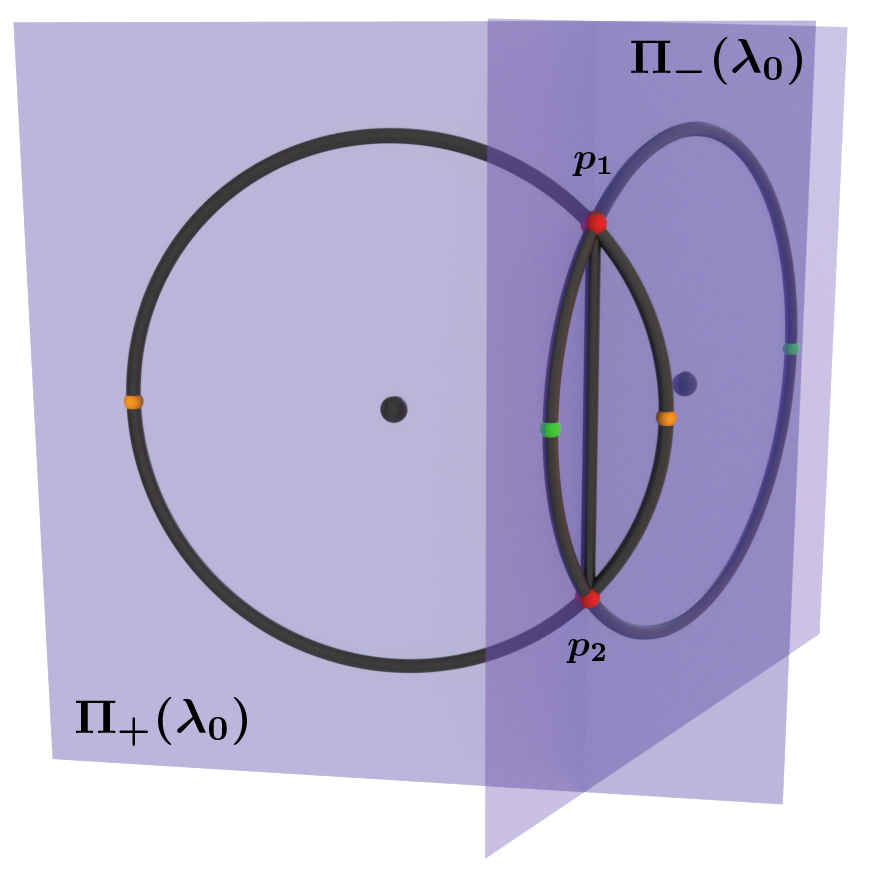
\includegraphics[width=0.42\textwidth]{proof_h2_side_view.png}
    \caption[The planes of the circular sections on two-sheeted hyperboloid.]{The planes of the circular sections on two-sheeted hyperboloid for a fixed $\lambda_{0}$. The orange and green points denote $q^{+}_{1,2}$ and $q^{-}_{1,2}$ respectively.}
    \label{fig:proof-h2}
\end{figure}

Once again, we extend Proposition~\ref{prop:affine-transformation-two-hyperboloid} to define a one-parameter family of curvature line parameterizations. We state the Theorem without proof, as it follows a similar approach to the proof of Theorem~\ref{thm:isometric-deformation-para-one-hyperboloid}.

\begin{theorem}
\label{thm:isometric-deformation-para-two-hyperboloid}
Let $a > b > c > 0$ and $\mathcal{H}(s_{1})$ be a one-parameter family of two-sheeted hyperboloids given by
\[
    \frac{b - c}{a - b} \frac{x^2}{\sin^2(s_{1})} - \frac{a - c}{a - b} \frac{y^2}{\cos^2(s_{1})} - z^2 = 1.
\]
Then for each $s_{1} \in \left[0, \frac{\pi}{2}\right]$ the two parameterizations
\begin{align*}
    \varphi_{\pm} &: [-s^{0}, s^{0}] \times [s^{0}, \infty) \to \mathbb{R}^3, \quad \quad (s_{2}, s_{3}) \mapsto (x, y, z) \\[10pt]
    x(s_{1}, s_{2}, s_{3}) &= \frac{a - b}{\sqrt{b - c} \sqrt{a - c}} \sin(s_{1}) \cosh(s_{2}) \cosh(s_{3}) \\[10 pt]
    y(s_{1}, s_{2}, s_{3}) &= \frac{a - b}{\sqrt{a - c} \sqrt{b - c}} \cos(s_{1}) \sinh(s_{2}) \sinh(s_{3}) \\[10 pt]
    z(s_{1}, s_{2}, s_{3}) &= \pm \sqrt{\frac{b - c}{a - c}} \sqrt{1 - \frac{a - b}{b - c} \sinh^2(s_{2})} \sqrt{\frac{a - b}{b - c} \sinh^2(s_{3}) - 1}
\end{align*}
with
\[
    s^{0} = \sinh^{-1}\left( \sqrt{ \frac{b - c}{a - b} } \right)
\]
are curvature line parameterizations of the two halves $\mathcal{H}(s_{1}) \cap \{ z \geq 0\}$ and $\mathcal{H}(s_{1}) \cap \{ z \leq 0\}$ of one sheet of the two-sheeted hyperboloid, and the curves $s_{2} \pm s_{3} = \text{const.}$ are congruent circles. \newline
This one-parameter family of one-sheeted hyperboloids $\mathcal{H}(s_{1})$ includes two planar degenerations corresponding to $s_{2} = 0,\left(x = 0 \right)$ and $s_{2} = \pi/2, \left(y = 0 \right)$.
\end{theorem}
\begin{figure}[H]
    \centering
    \includegraphics[width=1.0\textwidth]{h2-deform.png}
    \caption[Isometric deformation of two-sheeted hyperboloid along circular sections.]{Diagonally related nets of curvature lines and circular sections on a two-sheeted hyperboloid and its isometric deformation along circular sections.}
    \label{fig:h2-deform}
\end{figure}
\pagebreak
%===========================================================
% THE END
%===========================================================
% Set page style to "tocstyle"
\pagestyle{tocstyle}
\addcontentsline{toc}{section}{Bibliography}
\bibliographystyle{alphaurl}
\bibliography{refs}
%===========================================================


\end{document}
